%%%%%%%%%%%%%%%%%%%%%%%%%%%%%%%%%%%%%%%%%
% Short Sectioned Assignment LaTeX Template Version 1.0 (5/5/12)
% This template has been downloaded from: http://www.LaTeXTemplates.com
% Original author:  Frits Wenneker (http://www.howtotex.com)
% License: CC BY-NC-SA 3.0 (http://creativecommons.org/licenses/by-nc-sa/3.0/)
%%%%%%%%%%%%%%%%%%%%%%%%%%%%%%%%%%%%%%%%%

%----------------------------------------------------------------------------------------
%	PACKAGES AND OTHER DOCUMENT CONFIGURATIONS
%----------------------------------------------------------------------------------------

\documentclass[paper=a4, fontsize=11pt]{scrartcl} % A4 paper and 11pt font size

% ---- Entrada y salida de texto -----

\usepackage[T1]{fontenc} % Use 8-bit encoding that has 256 glyphs
\usepackage[utf8]{inputenc}
%\usepackage{fourier} % Use the Adobe Utopia font for the document - comment this line to return to the LaTeX default

% ---- Idioma --------

\usepackage[spanish, es-tabla]{babel} % Selecciona el español para palabras introducidas automáticamente, p.ej. "septiembre" en la fecha y especifica que se use la palabra Tabla en vez de Cuadro

% ---- Otros paquetes ----

\usepackage{url} % ,href} %para incluir URLs e hipervínculos dentro del texto (aunque hay que instalar href)
\usepackage{amsmath,amsfonts,amsthm} % Math packages
%\usepackage{graphics,graphicx, floatrow} %para incluir imágenes y notas en las imágenes
\usepackage{graphics,graphicx, float} %para incluir imágenes y colocarlas
% Para hacer cuadros
\usepackage{tcolorbox}
% Para hacer uso de párrafos
\usepackage{parskip}
\usepackage{hyperref}
\usepackage{vmargin}
\usepackage{amssymb}
\usepackage{indentfirst}

\setpapersize{A4}
\setmargins{2.5cm}       % margen izquierdo
{1.5cm}                        % margen superior
{16.5cm}                      % anchura del texto
{23.42cm}                    % altura del texto
{10pt}                           % altura de los encabezados
{1cm}                           % espacio entre el texto y los encabezados
{0pt}                             % altura del pie de página
{2cm}                           % espacio entre el texto y el pie de página
% Para hacer tablas comlejas
%\usepackage{multirow}
%\usepackage{threeparttable}

%\usepackage{sectsty} % Allows customizing section commands
%\allsectionsfont{\centering \normalfont\scshape} % Make all sections centered, the default font and small caps

\usepackage{fancyhdr} % Custom headers and footers
\pagestyle{fancyplain} % Makes all pages in the document conform to the custom headers and footers
\fancyhead{} % No page header - if you want one, create it in the same way as the footers below
\fancyfoot[L]{Marina Muñoz Cano y Mario López González 3ºB1} % Empty left footer
\fancyfoot[C]{} % Empty center footer
\fancyfoot[R]{\thepage} % Page numbering for right footer
\renewcommand{\headrulewidth}{0pt} % Remove header underlines
\renewcommand{\footrulewidth}{0pt} % Remove footer underlines
\setlength{\headheight}{13.6pt} % Customize the height of the header

\numberwithin{equation}{section} % Number equations within sections (i.e. 1.1, 1.2, 2.1, 2.2 instead of 1, 2, 3, 4)
\numberwithin{figure}{section} % Number figures within sections (i.e. 1.1, 1.2, 2.1, 2.2 instead of 1, 2, 3, 4)
\numberwithin{table}{section} % Number tables within sections (i.e. 1.1, 1.2, 2.1, 2.2 instead of 1, 2, 3, 4)

\setlength\parindent{0pt} % Removes all indentation from paragraphs - comment this line for an assignment with lots of text

\newcommand{\horrule}[1]{\rule{\linewidth}{#1}} % Create horizontal rule command with 1 argument of height


\title{	
\normalfont \normalsize 
\textsc{\textbf{Modelos de Computación} \\ Grado en Ingeniería Informática \\ Universidad de Granada} \\ [25pt] % Your university, school and/or department name(s)
\horrule{0.5pt} \\[0.4cm] % Thin top horizontal rule
\huge Memoria Prácticas \\ % The assignment title
\horrule{2pt} \\[0.5cm] % Thick bottom horizontal rule
}

% Nombre y apellidos
\author{ 
    Marina Muñoz Cano
    \\
    Mario López González
} 

\date{\normalsize\today} % Incluye la fecha actual

%----------------------------------------------------------------------------------------
% DOCUMENTO
%----------------------------------------------------------------------------------------

\begin{document}

\maketitle % Muestra el Título

\newpage %inserta un salto de página

\tableofcontents % para generar el índice de contenidos
\listoffigures % para generar el índice de imágenes

\newpage

\section{Practica 1 - Relación Ejercicios 1b}

\subsection{Ejercicios Sencillos}

\textbf{a)}  $\{ u \in \{0,1\}^{\ast} $ tales que $\mid u \mid$ $\leq 4 \}$

\begin{figure}[H] 
	\centering
	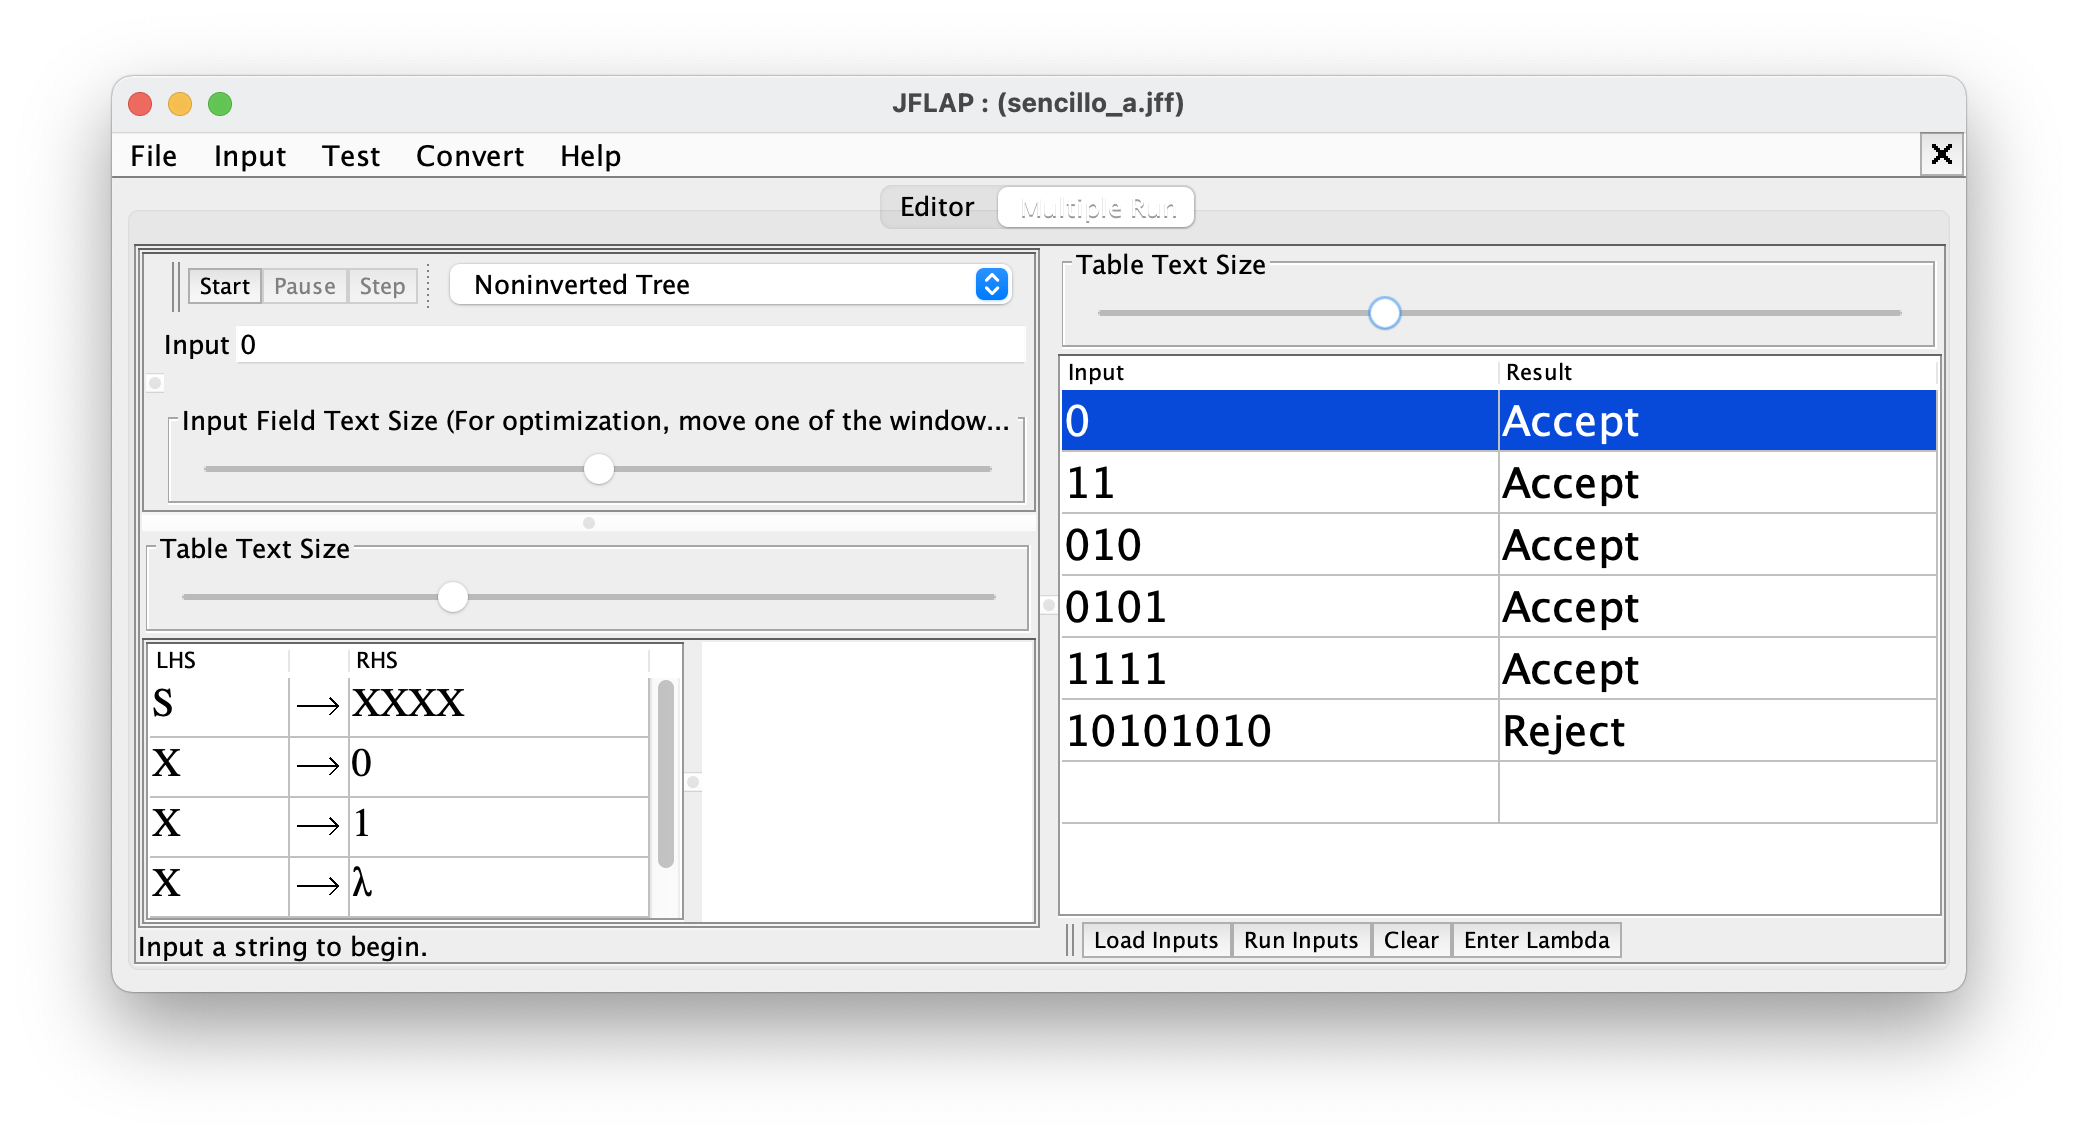
\includegraphics[scale=0.35]{../practica_1/images/sencillo_a.png} 
	\caption{Sencillo a en JFLAP} 
    \label{fig:sencillo_a}
\end{figure}

Usamos una variable X que puede tomar valor 0, 1 o $\varepsilon$, como son palabras de 0's y 1's de longitud menor o igual que 4, 
el simbolo de partida son cuatro X's. De esta forma se aceptan cadenas de longitud 4 o menos, ya que X puede tomar el valor $\varepsilon$. \\

\textbf{b)}  Palabras con 0's y 1's que no contengan dos 1's consecutivos y que empiecen por un 1 y que terminen por dos 0's.

\begin{figure}[H] 
	\centering
	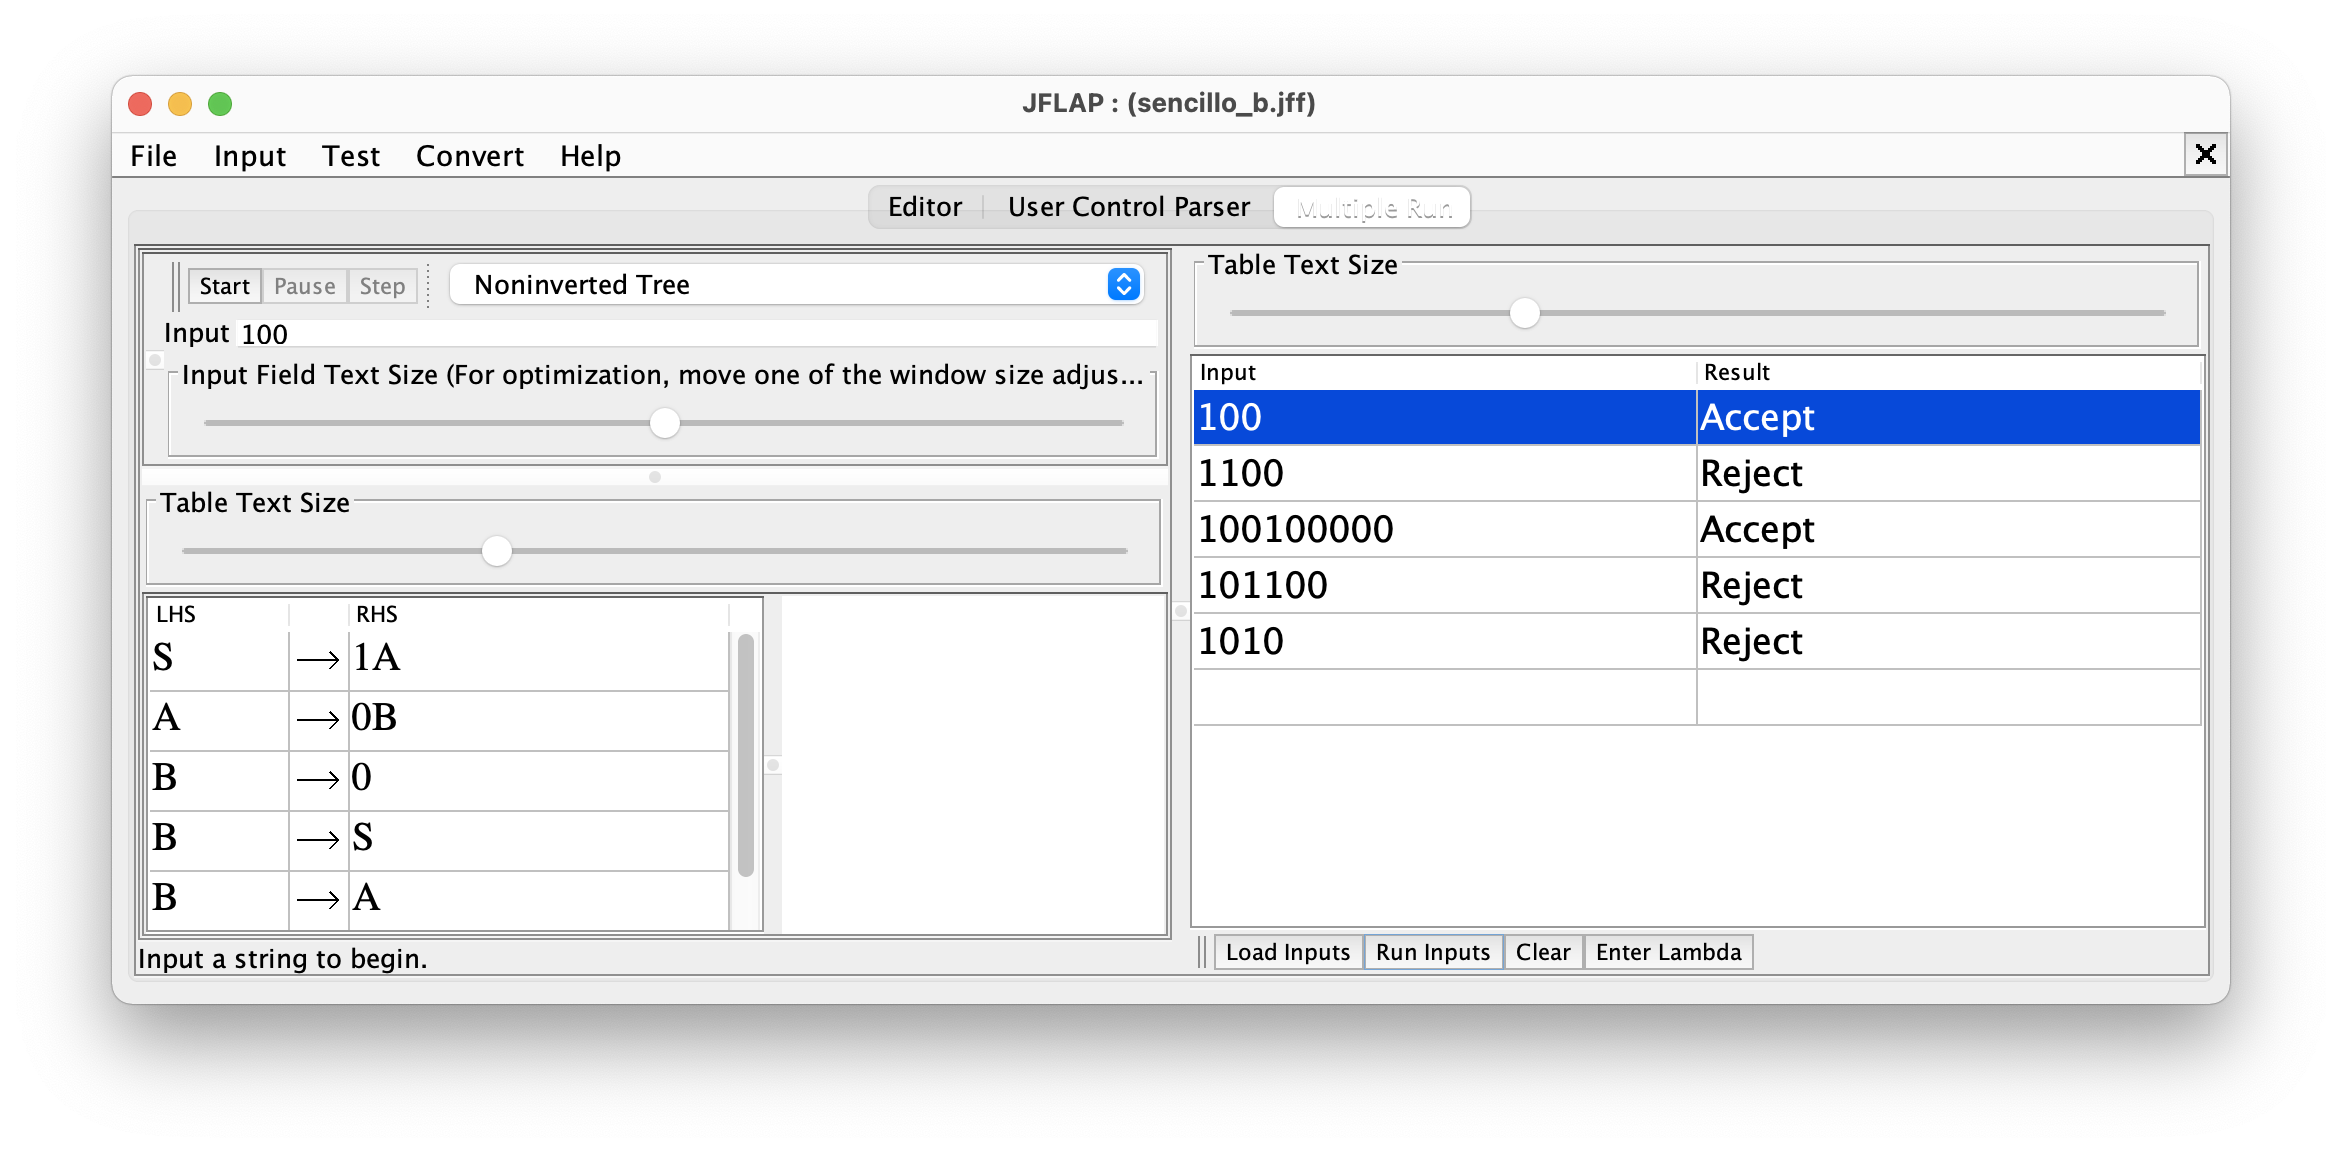
\includegraphics[scale=0.35]{../practica_1/images/sencillo_b.png} 
	\caption{Sencillo b en JFLAP} 
    \label{fig:sencillo_b}
\end{figure}

La variable A añade 0's tras añadir un 1, para que no contenga dos consecutivos. La variable B va generando el resto de la cadena (Añadiendo 0's o 1)
de forma que la unica forma de acabar la cadena es cuando B vale 0, es decir, con dos 0 consecutivos. 
\\

\textbf{c)}  El conjunto vacío. 

\begin{figure}[H] 
	\centering
	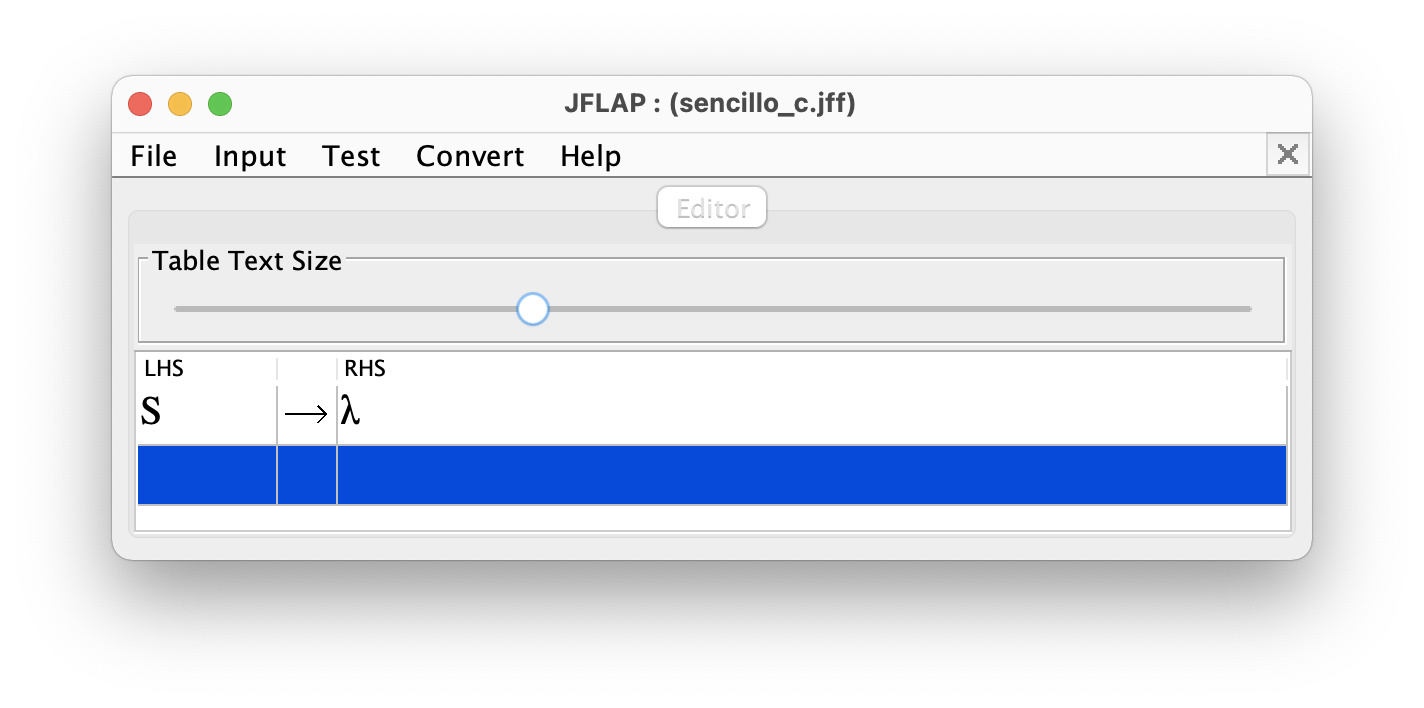
\includegraphics[scale=0.5]{../practica_1/images/sencillo_c.png} 
	\caption{Sencillo c en JFLAP} 
    \label{fig:sencillo_c}
\end{figure}

No mostramos ejemplos, ya que JFLAP no nos lo permite, al no detectar ningun simbolo como terminal.

\begin{figure}[H] 
	\centering
	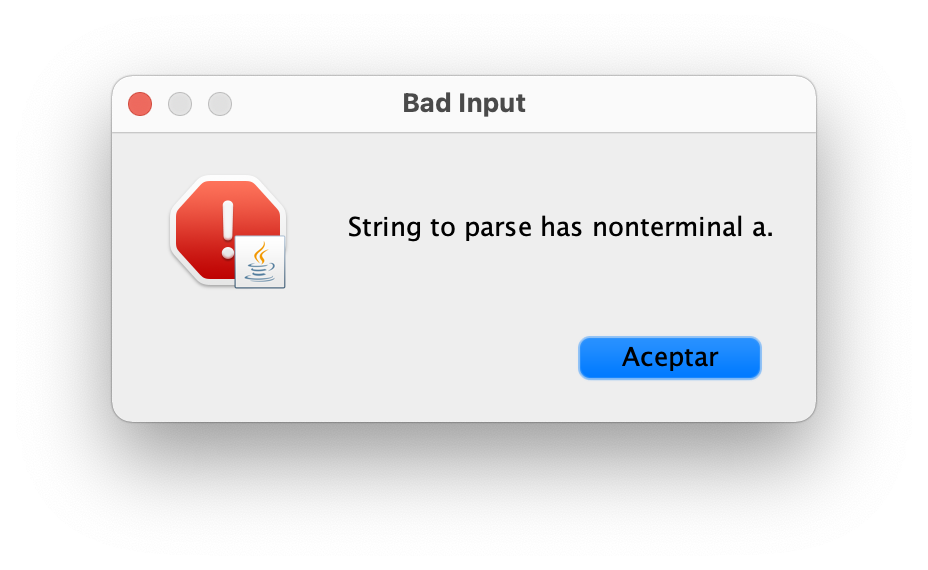
\includegraphics[scale=0.5]{../practica_1/images/sencillo_c_err.png} 
	\caption{Sencillo c error en JFLAP} 
    \label{fig:sencillo_c_err}
\end{figure}

\textbf{d)}  El lenguaje formado por los números naturales.

El lenguaje genera las cifras del numero final de izquierda a derecha, no puediendo empezar por 0. De esta forma generamos un número que comprende
entre el 1 y el 9. Tras esto se le puede agregar cualquier número entre 0 y 9.

\begin{figure}[H] 
	\centering
	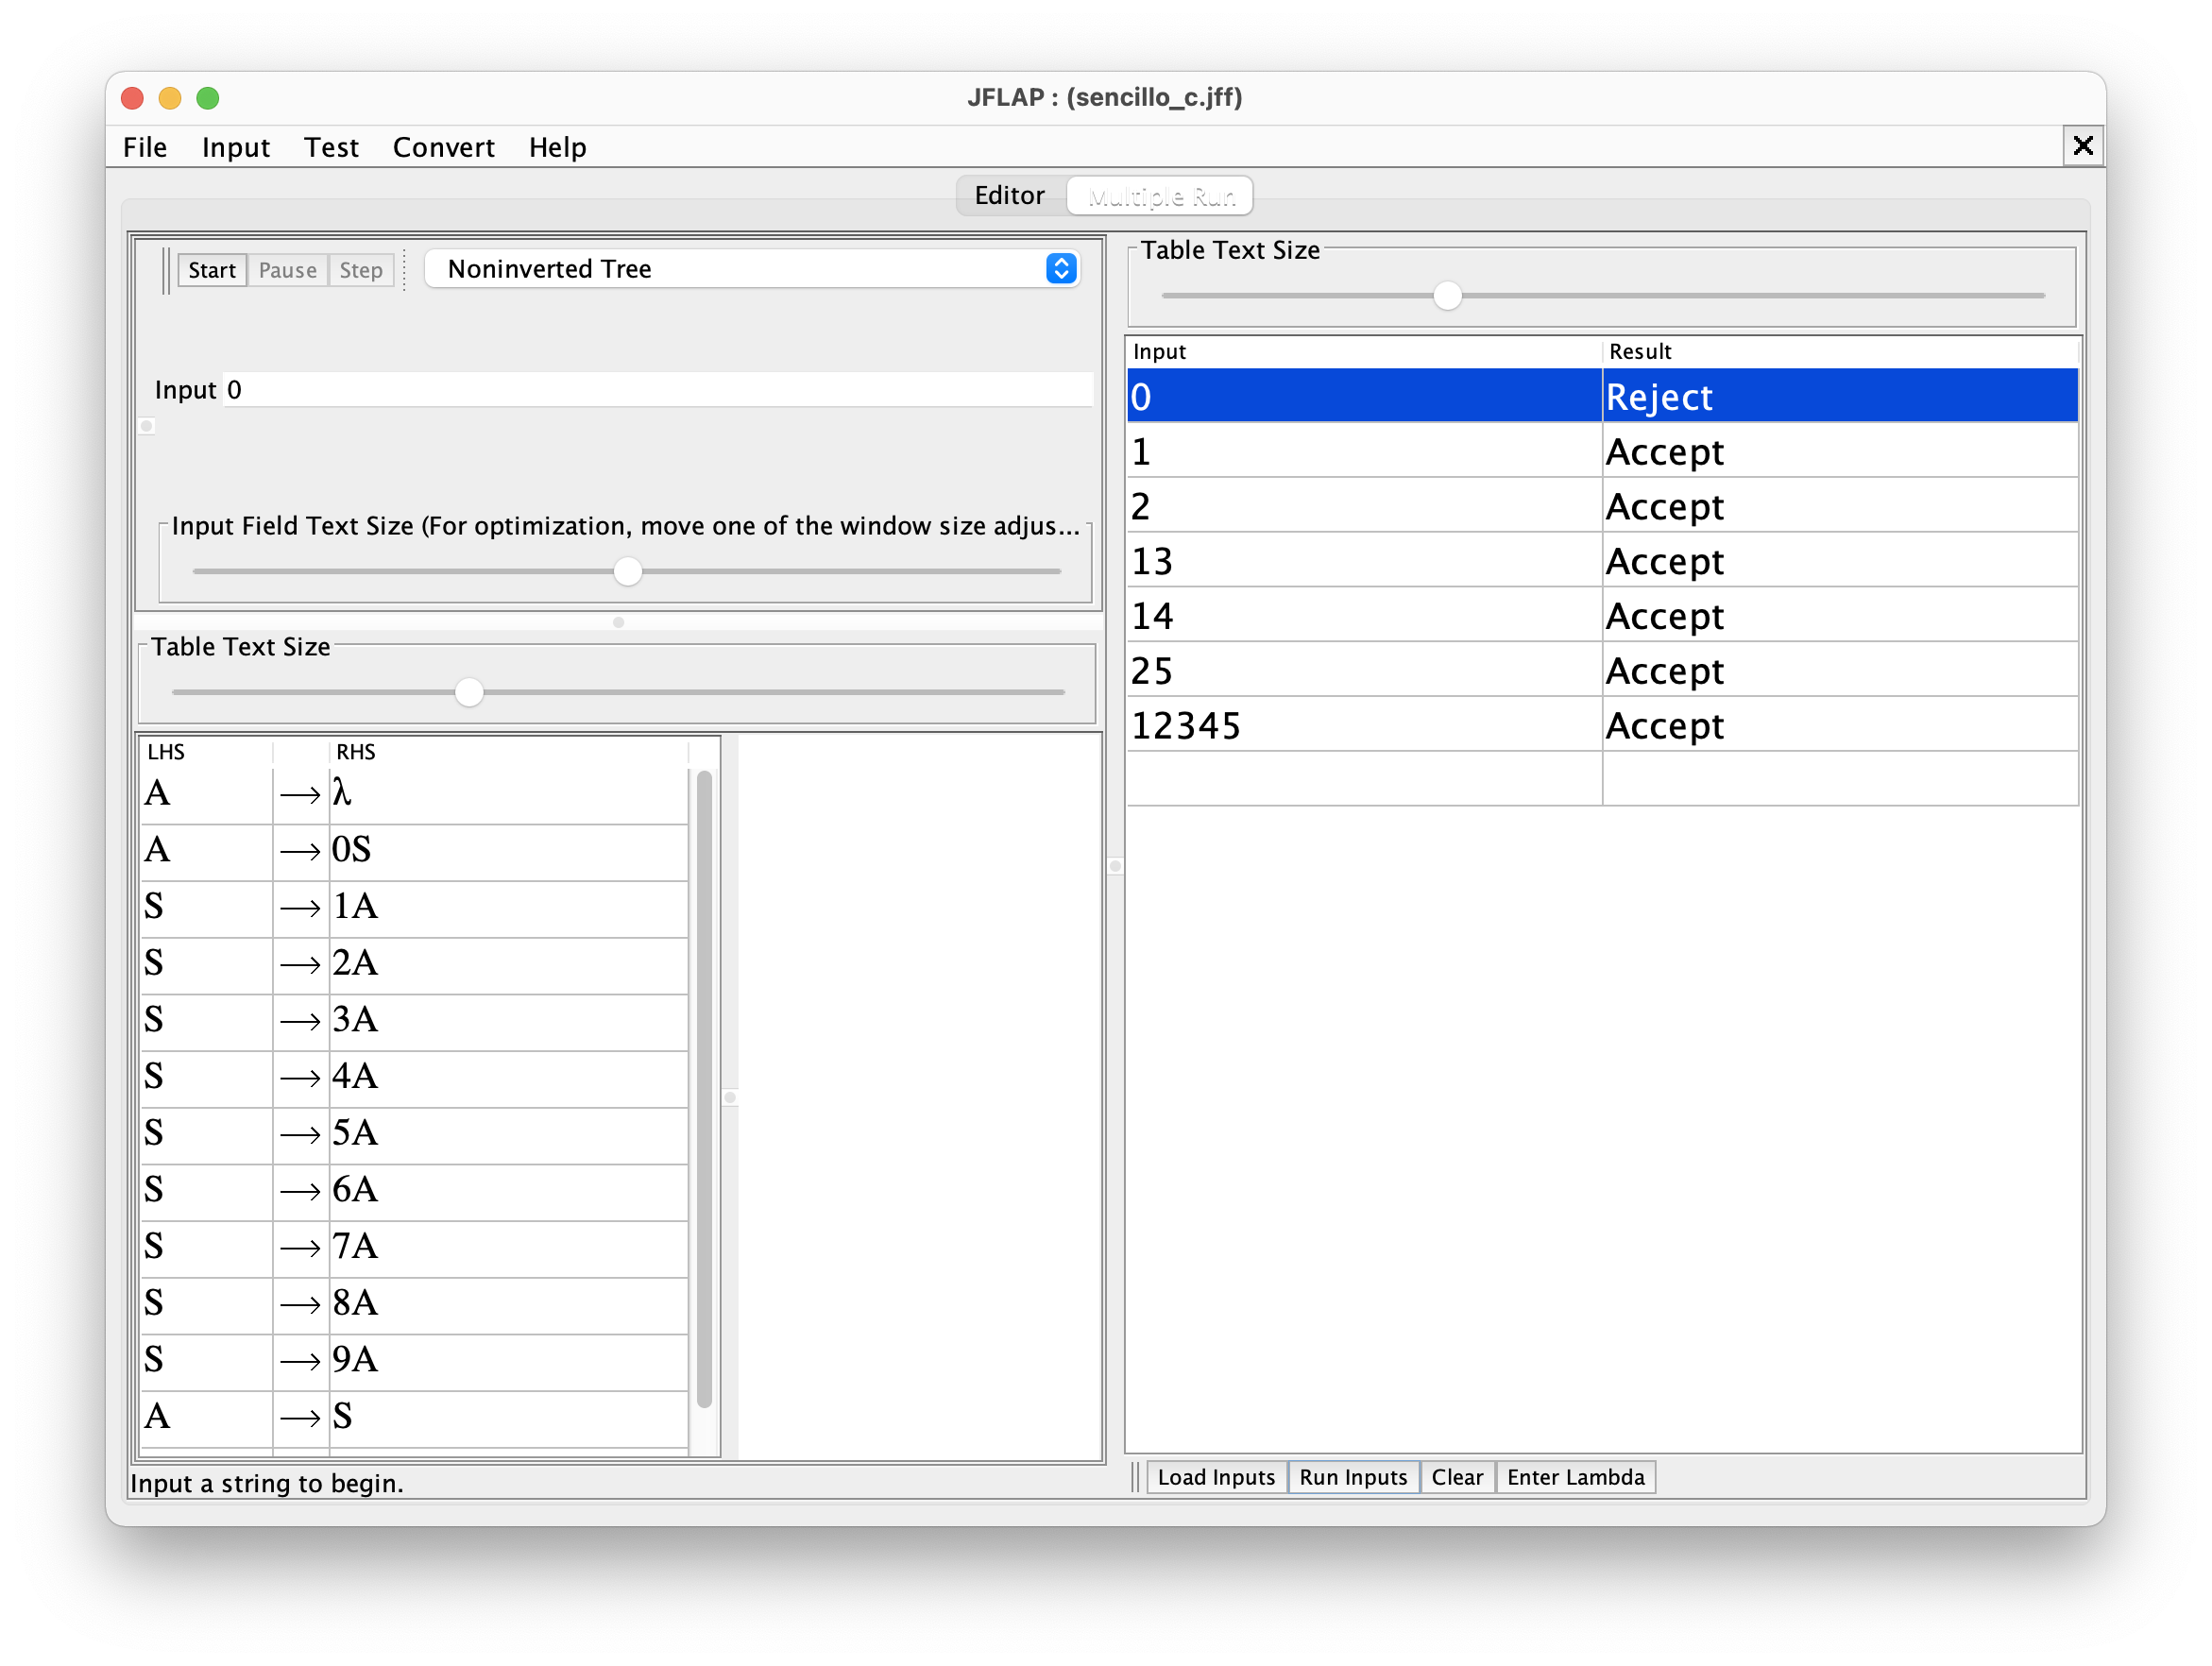
\includegraphics[scale=0.35]{../practica_1/images/sencillo_d.png} 
	\caption{Sencillo d en JFLAP} 
    \label{fig:sencillo_d}
\end{figure}

\textbf{f)}  $\{ a^{n} b^{2n} c^{m} \in \{a,b,c\}^{\ast}$ con $n,m > 0\}$

Con la variable A, por cada a generamos dos b's. Tras generar las n a's y las 2n b's generamos m c's con la variable C.

\begin{figure}[H] 
	\centering
	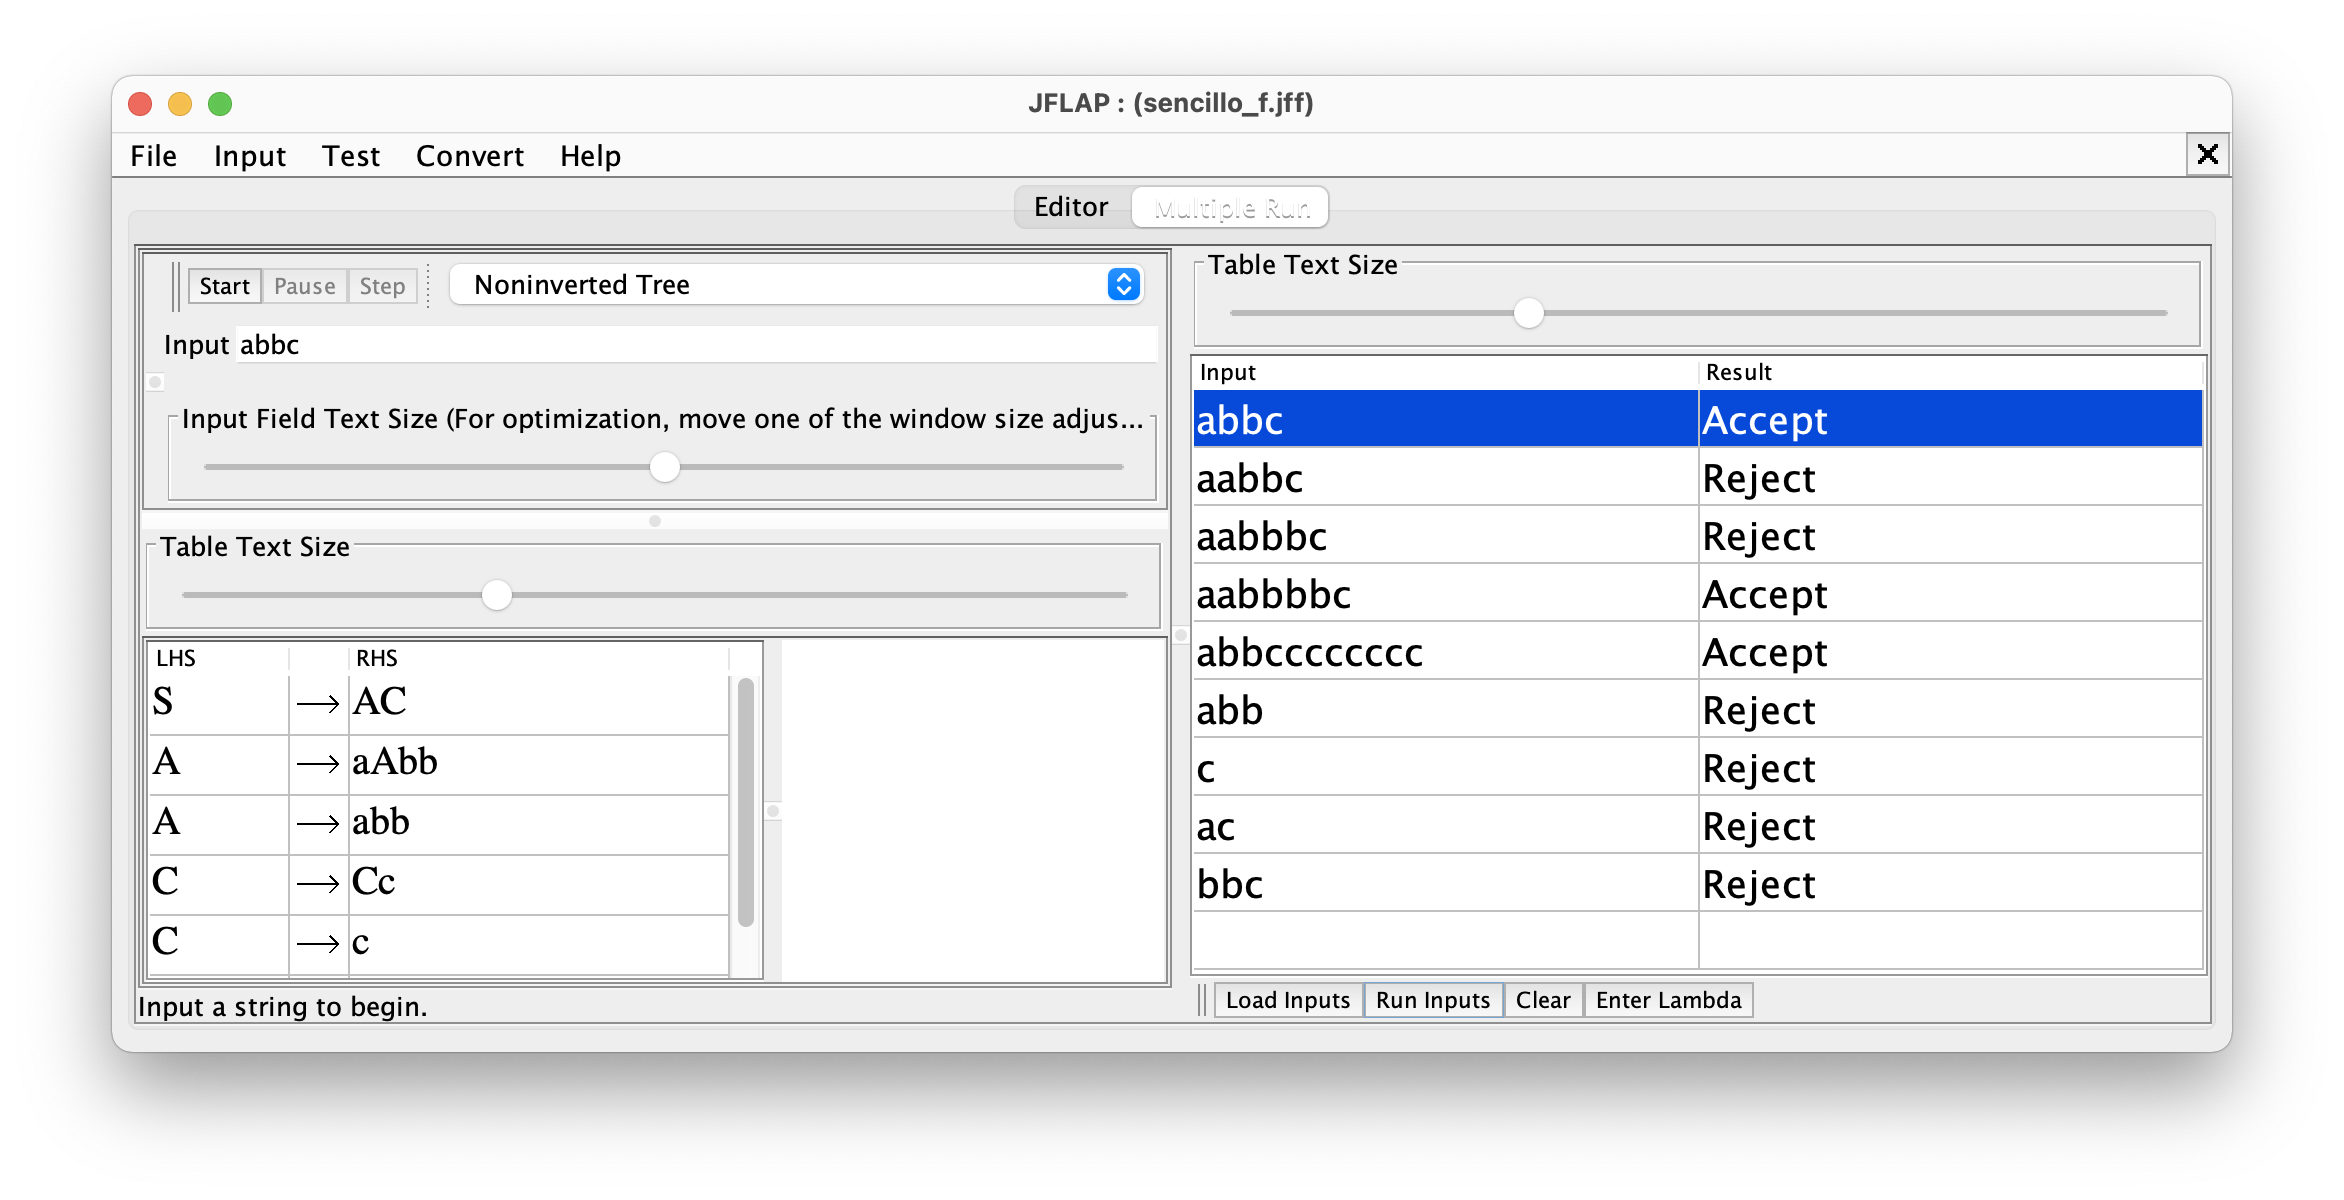
\includegraphics[scale=0.35]{../practica_1/images/sencillo_f.png} 
	\caption{Sencillo f en JFLAP} 
    \label{fig:sencillo_f}
\end{figure}

\textbf{g)} $\{ a^{n} b^{m} a^{n} \in \{a,b\}^{\ast}$ con $m,n > 0\}$

Con el símbolo de partida S, generamos el número de a's mínimo que admite el lenguaje. Tras esto se puede seguir añadiendo a's a ambos lados o incluir las m b's,
siendo obligatorio añadir como mínimo una b. 

\begin{figure}[H] 
	\centering
	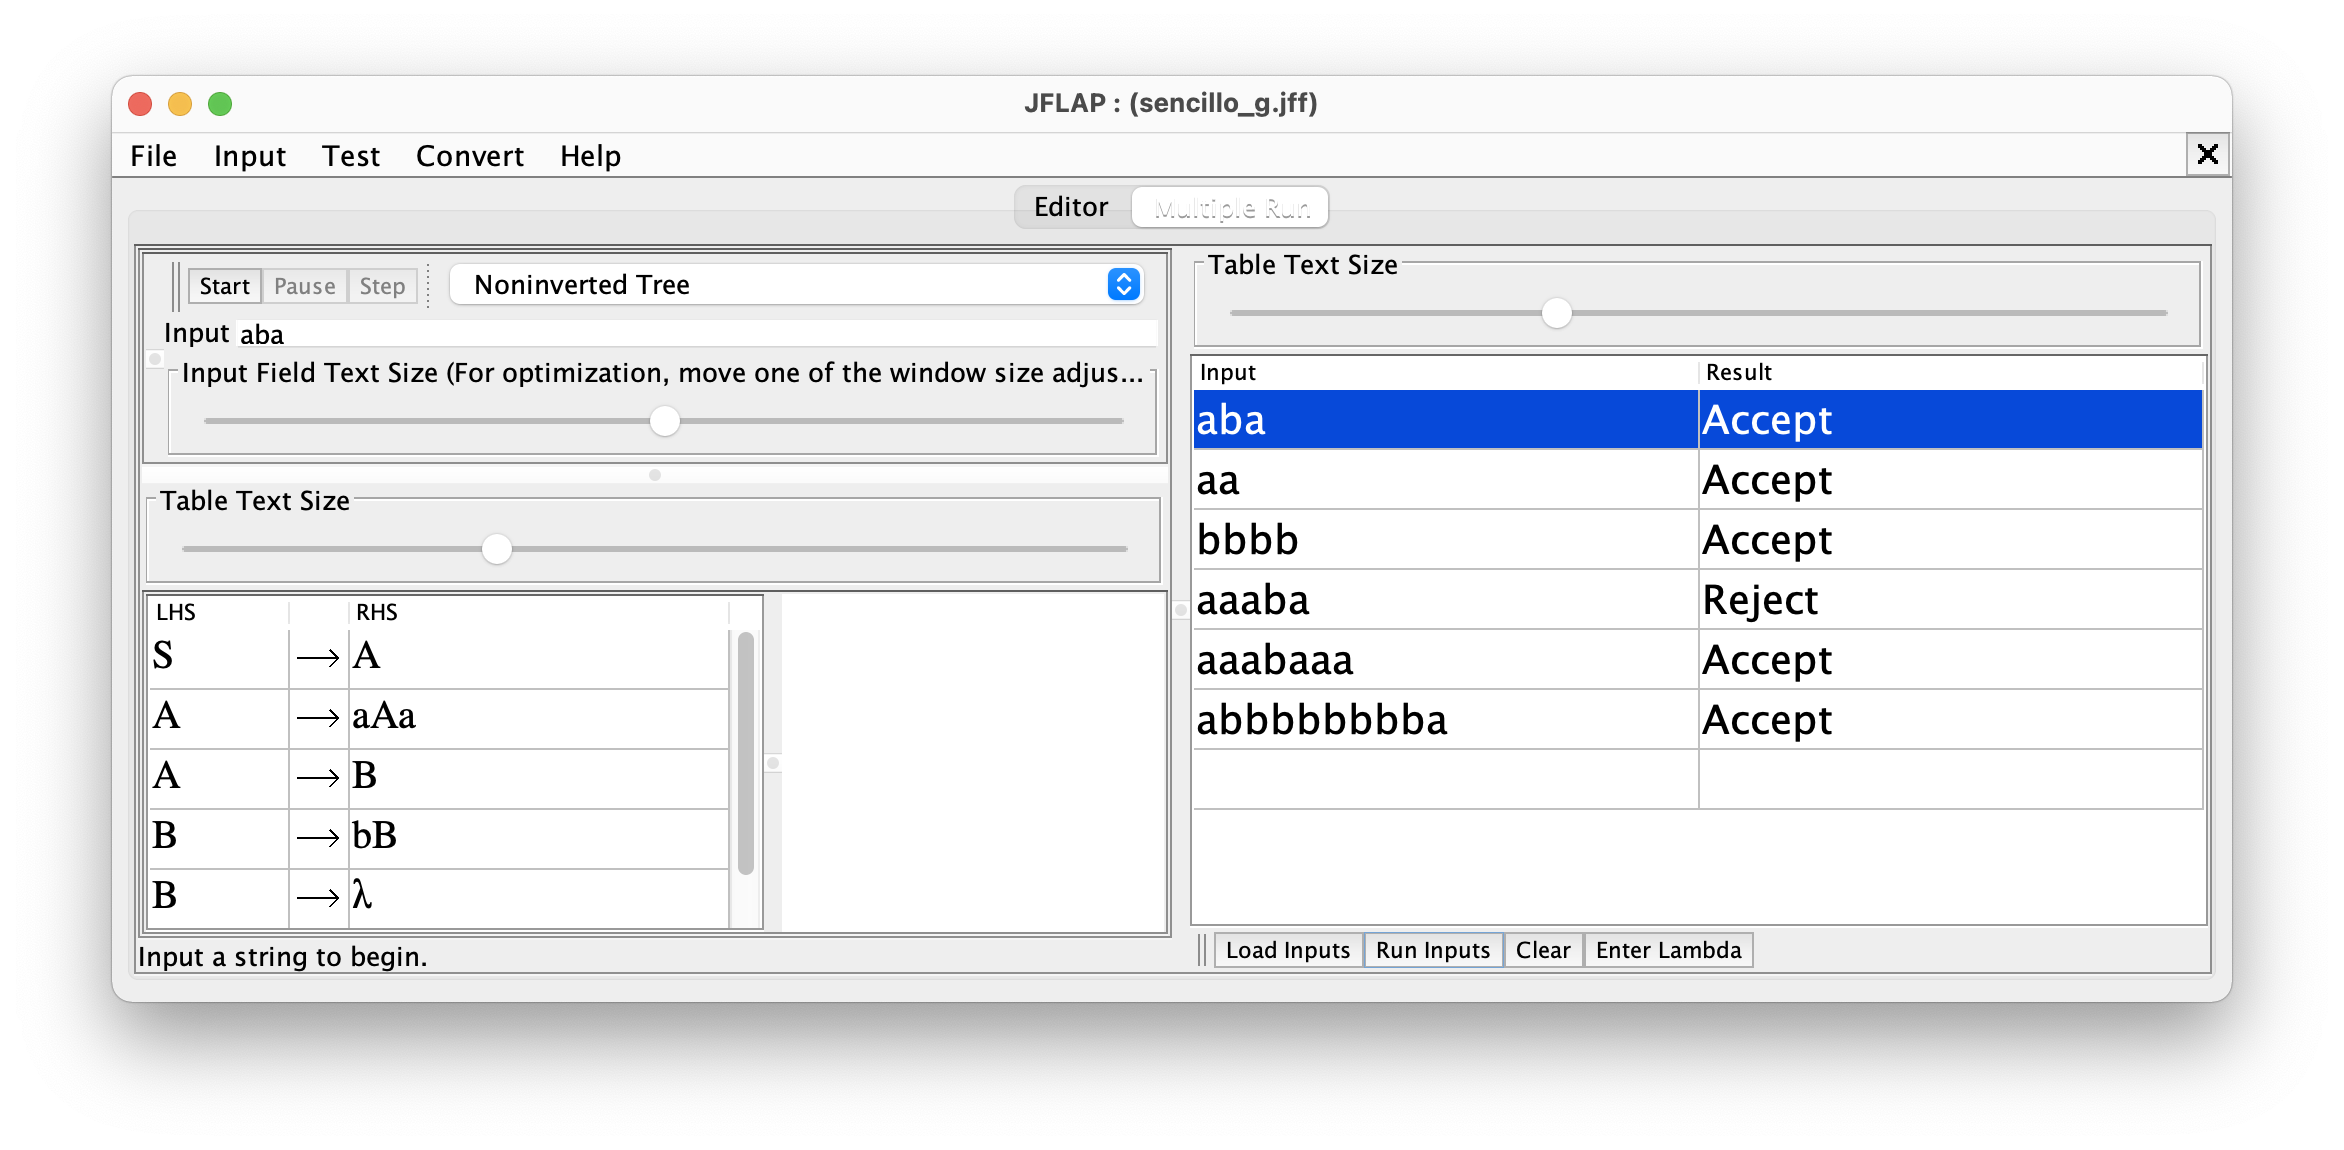
\includegraphics[scale=0.4]{../practica_1/images/sencillo_g.png} 
	\caption{Sencillo g en JFLAP} 
    \label{fig:sencillo_g}
\end{figure}

\textbf{h)}  Palabras con 0's y 1's que contengan la subcadena 00 y 11.

\begin{figure}[H] 
	\centering
	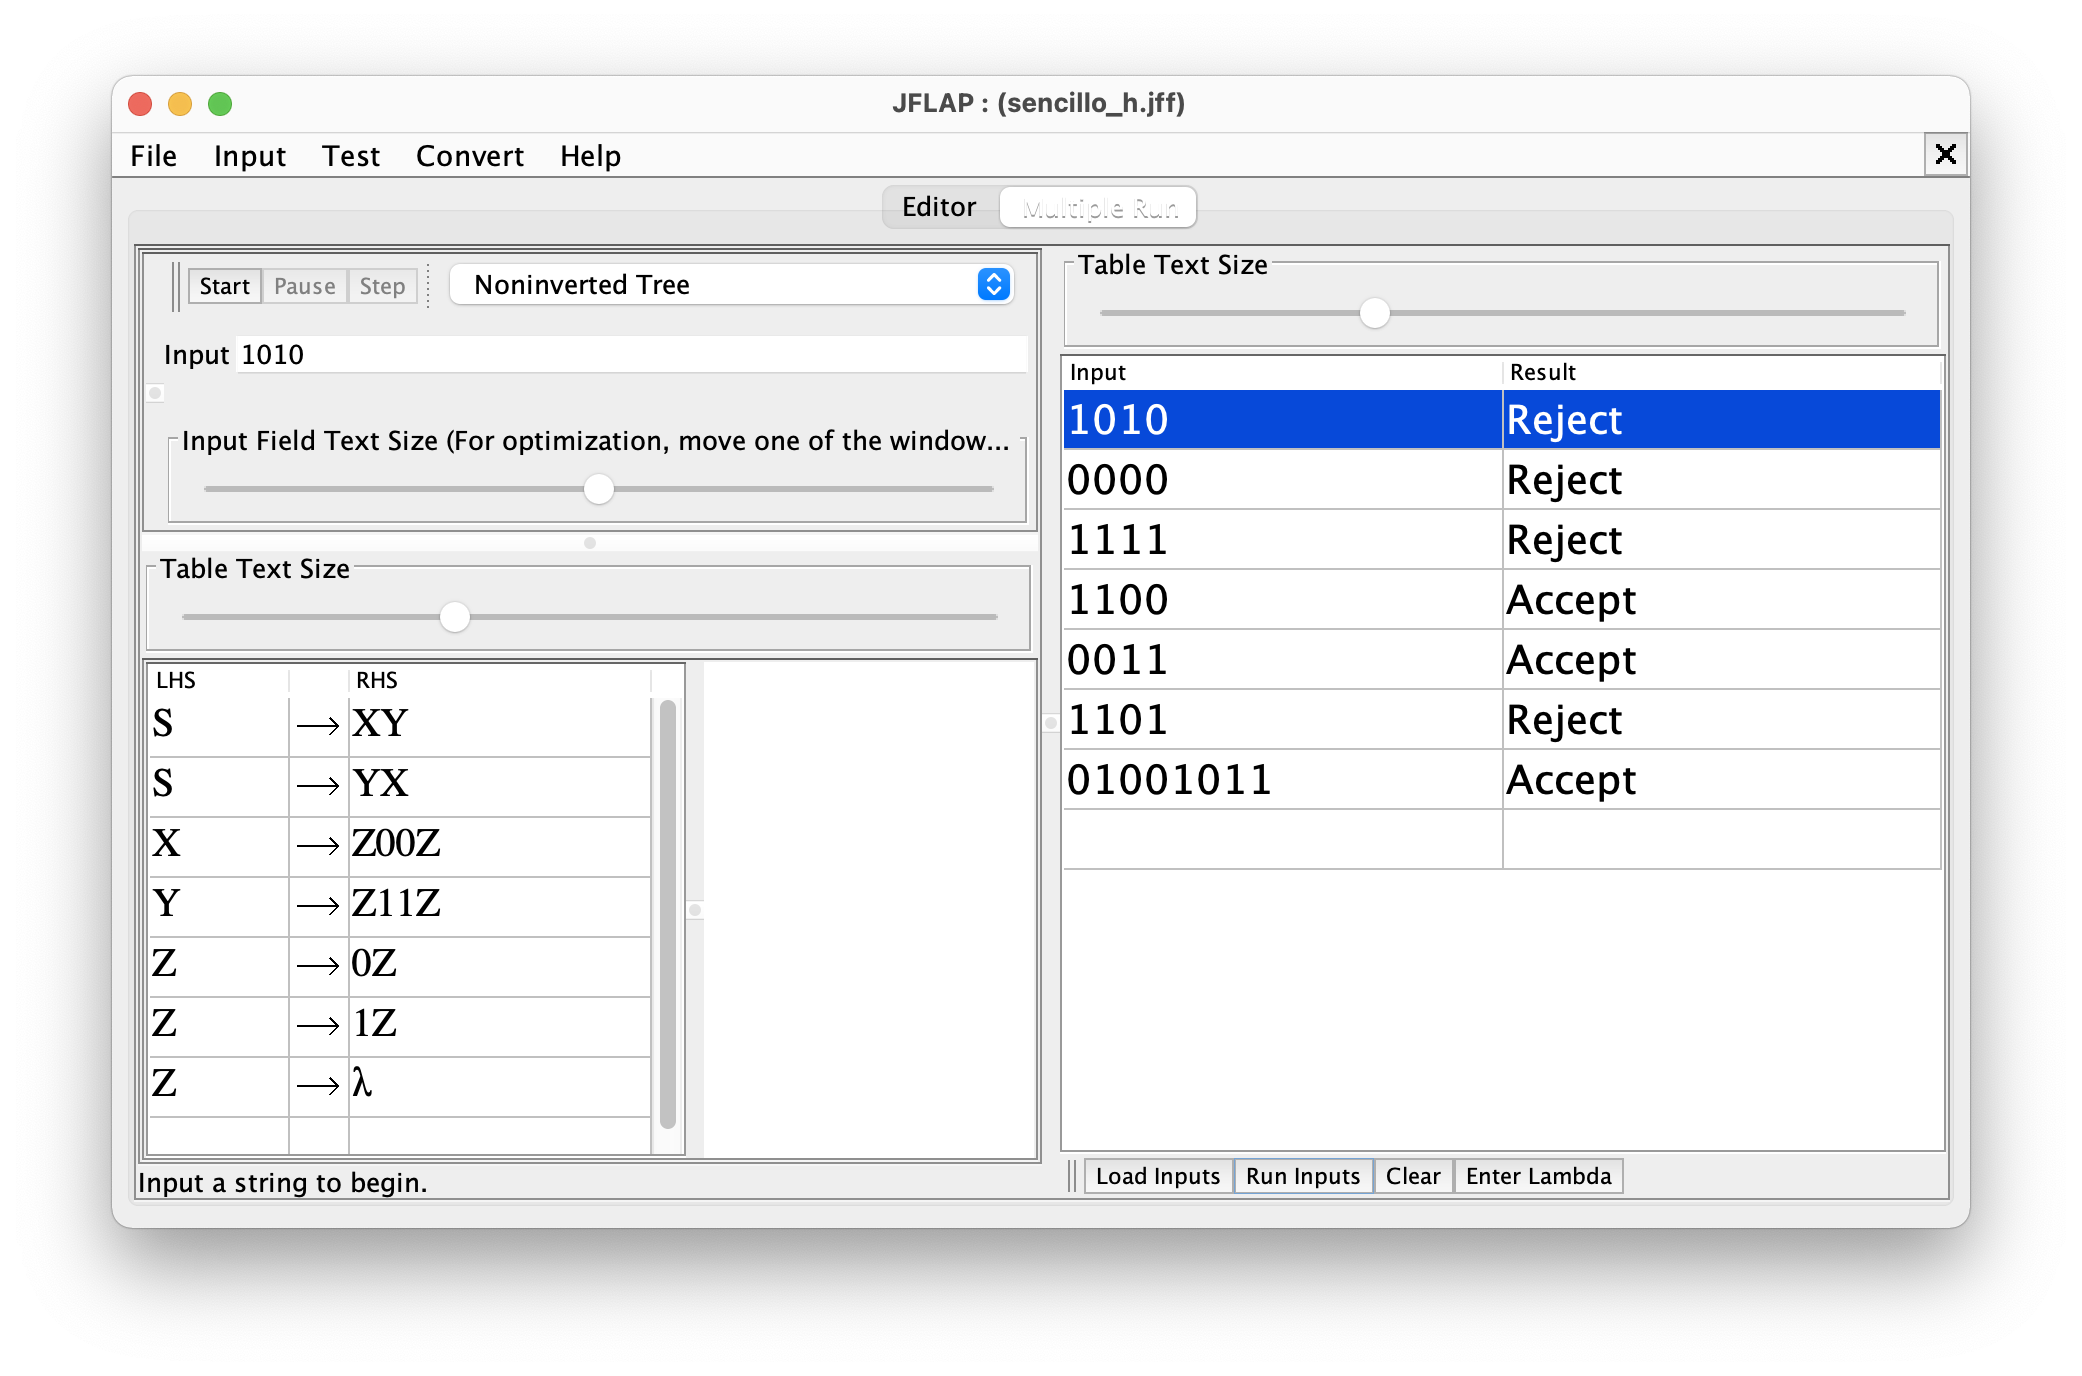
\includegraphics[scale=0.35]{../practica_1/images/sencillo_h.png} 
	\caption{Sencillo h en JFLAP} 
    \label{fig:sencillo_h}
\end{figure}

Con las variables S generamos las dos subcadenas necesarias, representadas por X e Y. Con las variables anteriores se añaden variables Z a ambos lados de las
cadenas, siendo posible sustituilas por 0's, 1's o $\varepsilon$. De esta forma, se generan cadenas de 0's y 1's que contienen en cualquier orden las subcadenas 00 y 11. \\

\textbf{i)}  Palíndromos formados con las letras a y b.

Para formar los palíndromos con el símbolo de partida generamos dos a's o dos b's. En las cadenas generadas incluimos la variable S para que se puedan generar las cadenas de 
a's y b's necesarias para crear el palíndromo. Además, incluimos las reglas de produccion que sustituyen S por a y b para poder generar palíndromos impares y otra regla,
S $\rightarrow$ $\varepsilon$, para generar pares.

\begin{figure}[H] 
	\centering
	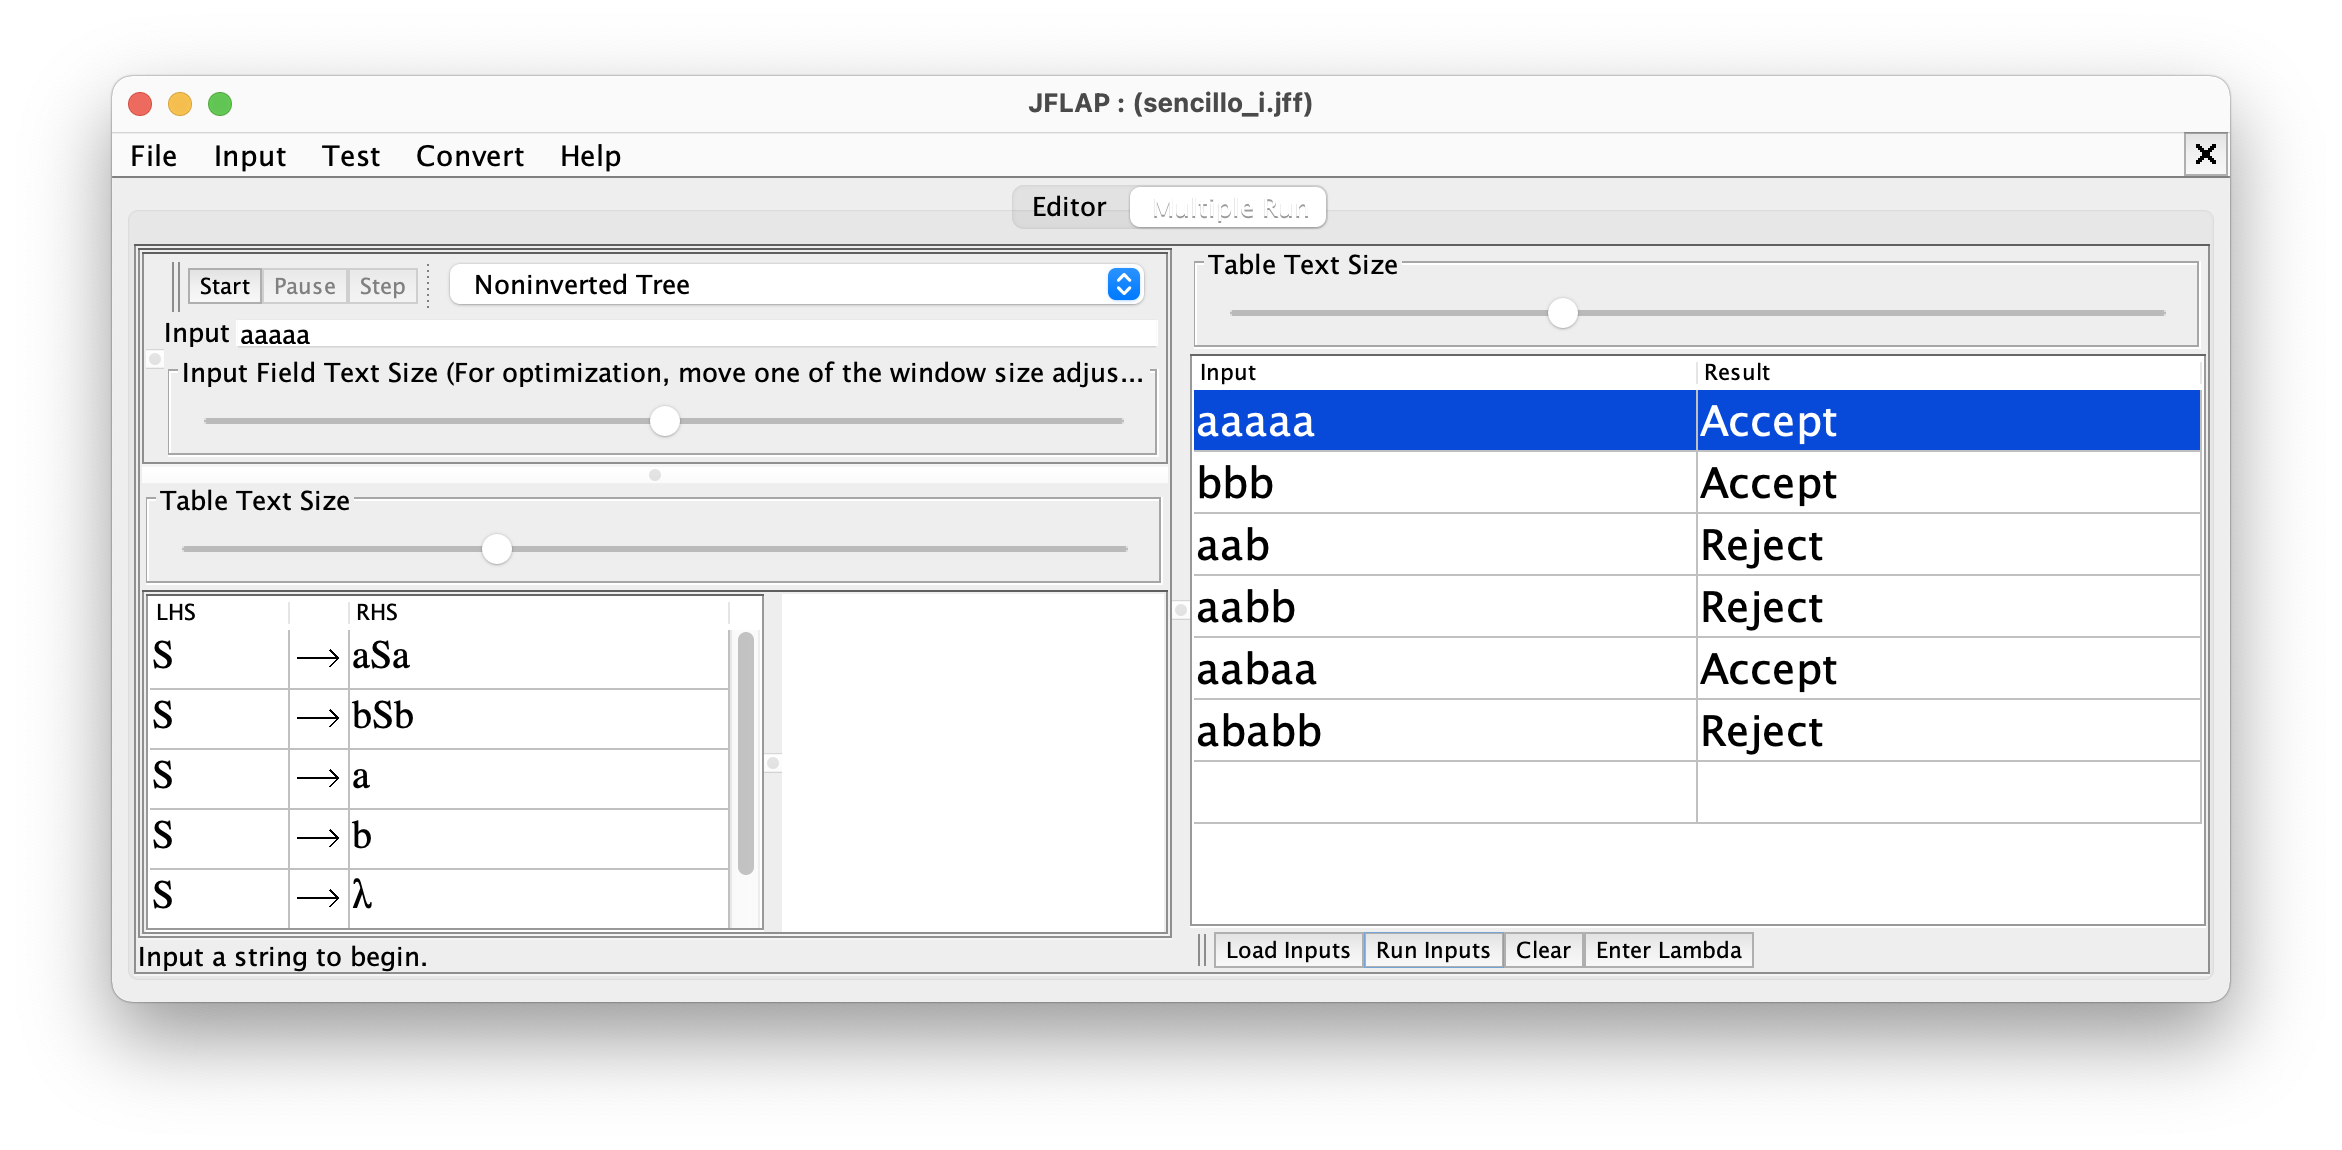
\includegraphics[scale=0.375]{../practica_1/images/sencillo_i.png} 
	\caption{Sencillo i en JFLAP} 
    \label{fig:sencillo_i}
\end{figure}

\newpage

\subsection{Ejercicios Intermedios}

\textbf{a)}  $\{ uv \in \{0,1\}^{\ast} $ tales que $u^{-1}$ es un prefijo de $v\}$

\begin{figure}[H] 
	\centering
	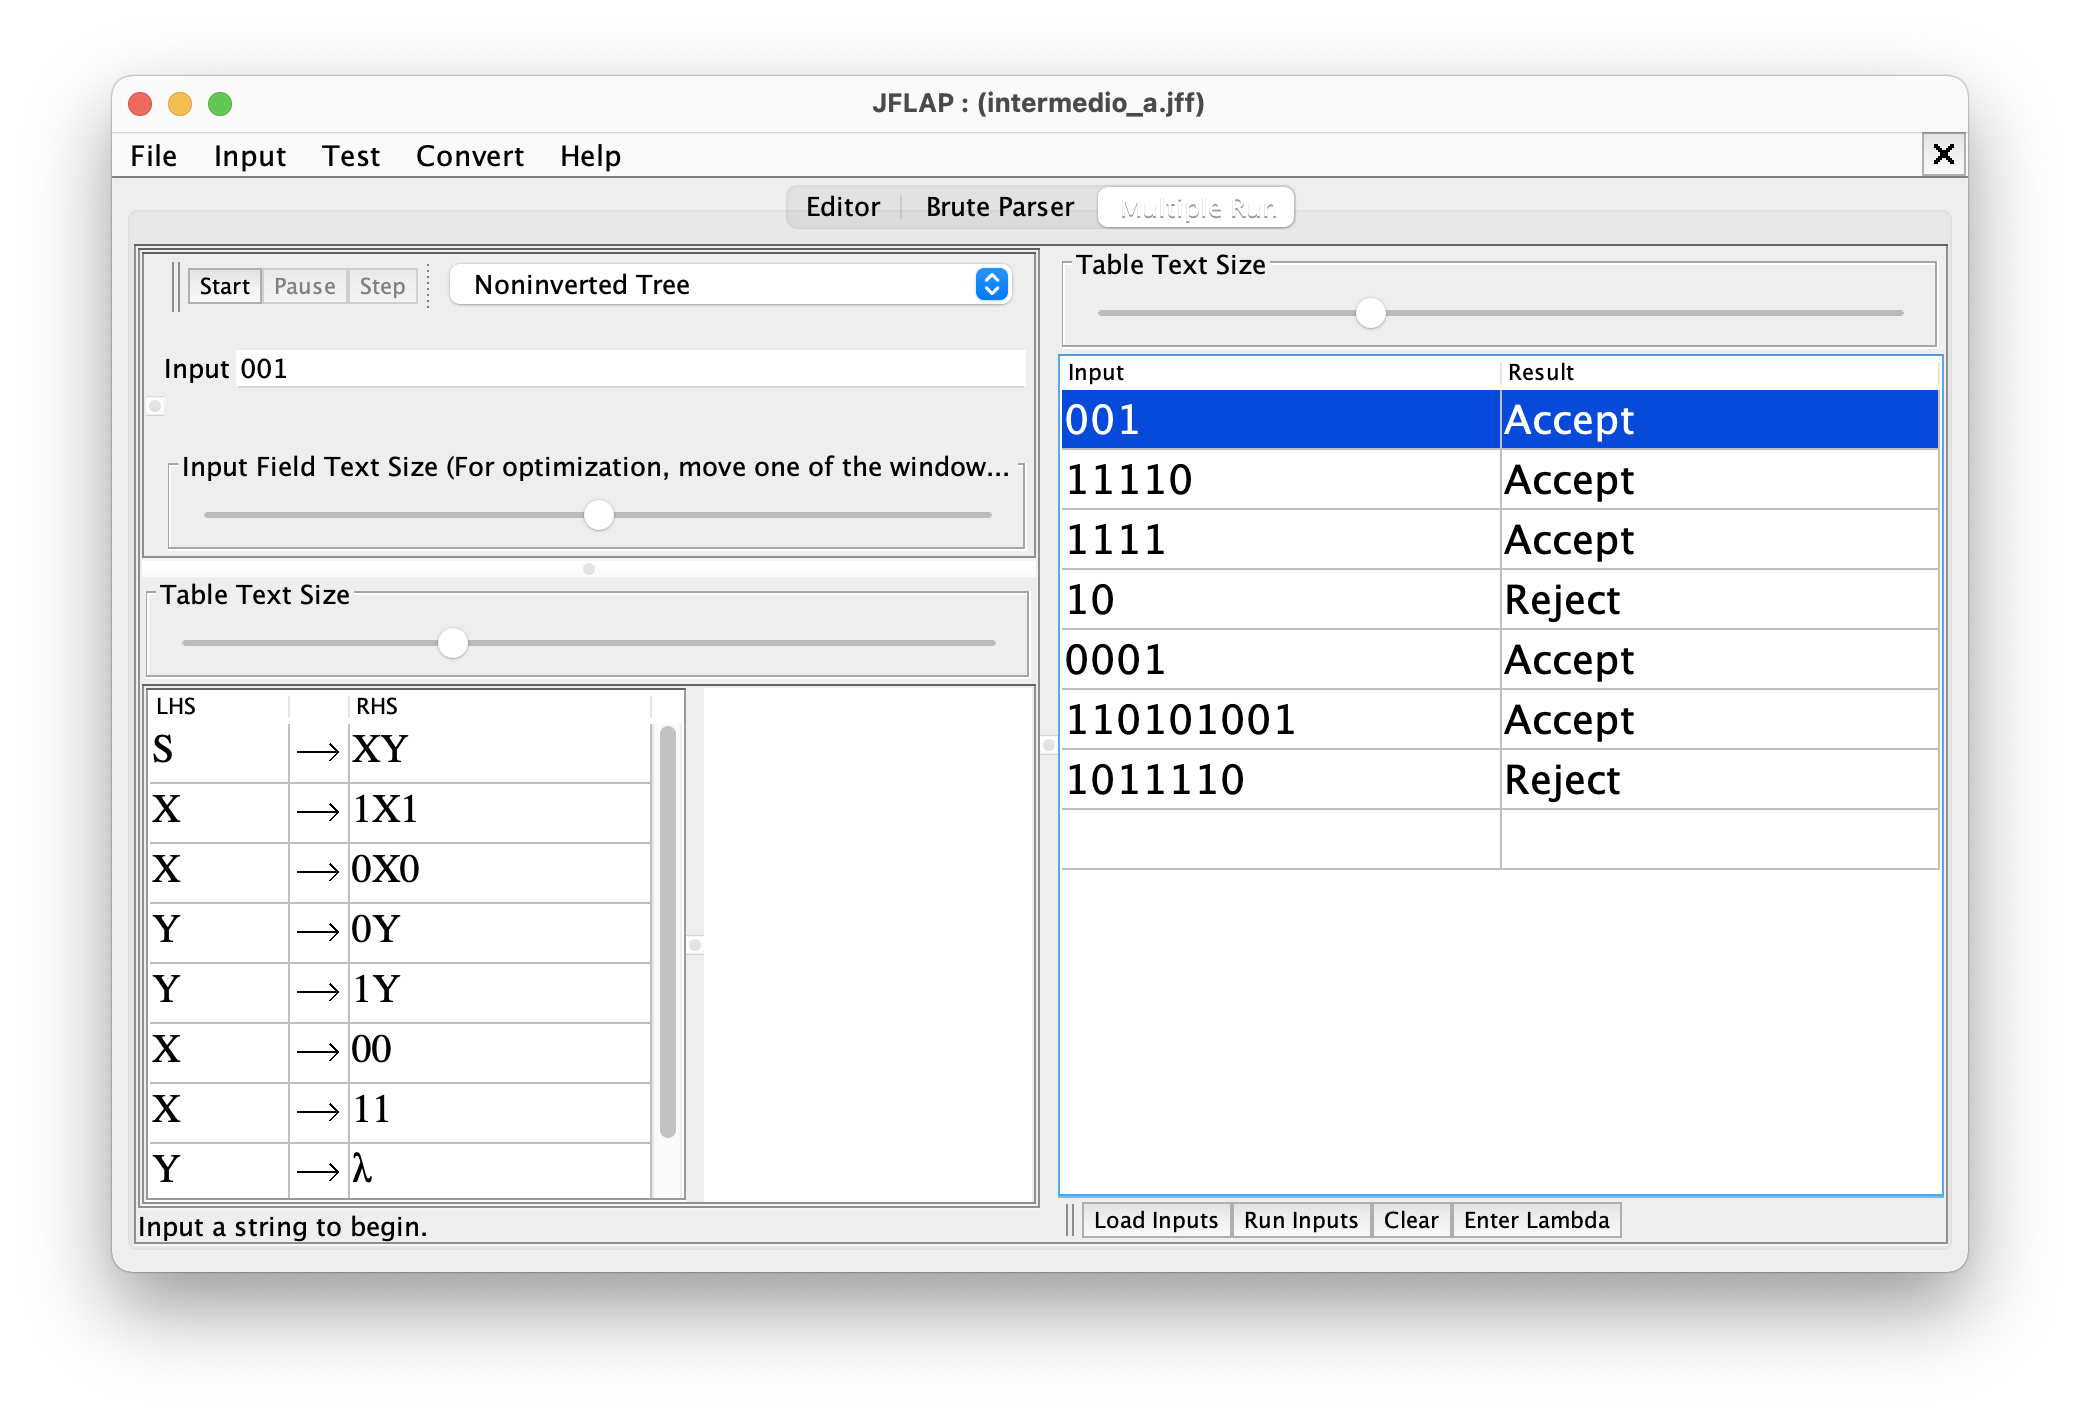
\includegraphics[scale=0.35]{../practica_1/images/intermedio_a.png} 
	\caption{Intermedio a en JFLAP} 
    \label{fig:intermedio_a}
\end{figure}

\textbf{b)}  $\{ ucv \in \{a,b,c\}^{\ast} $ tales que $u$ y $v$ tienen la misma longitud$\}$

\begin{figure}[H] 
	\centering
	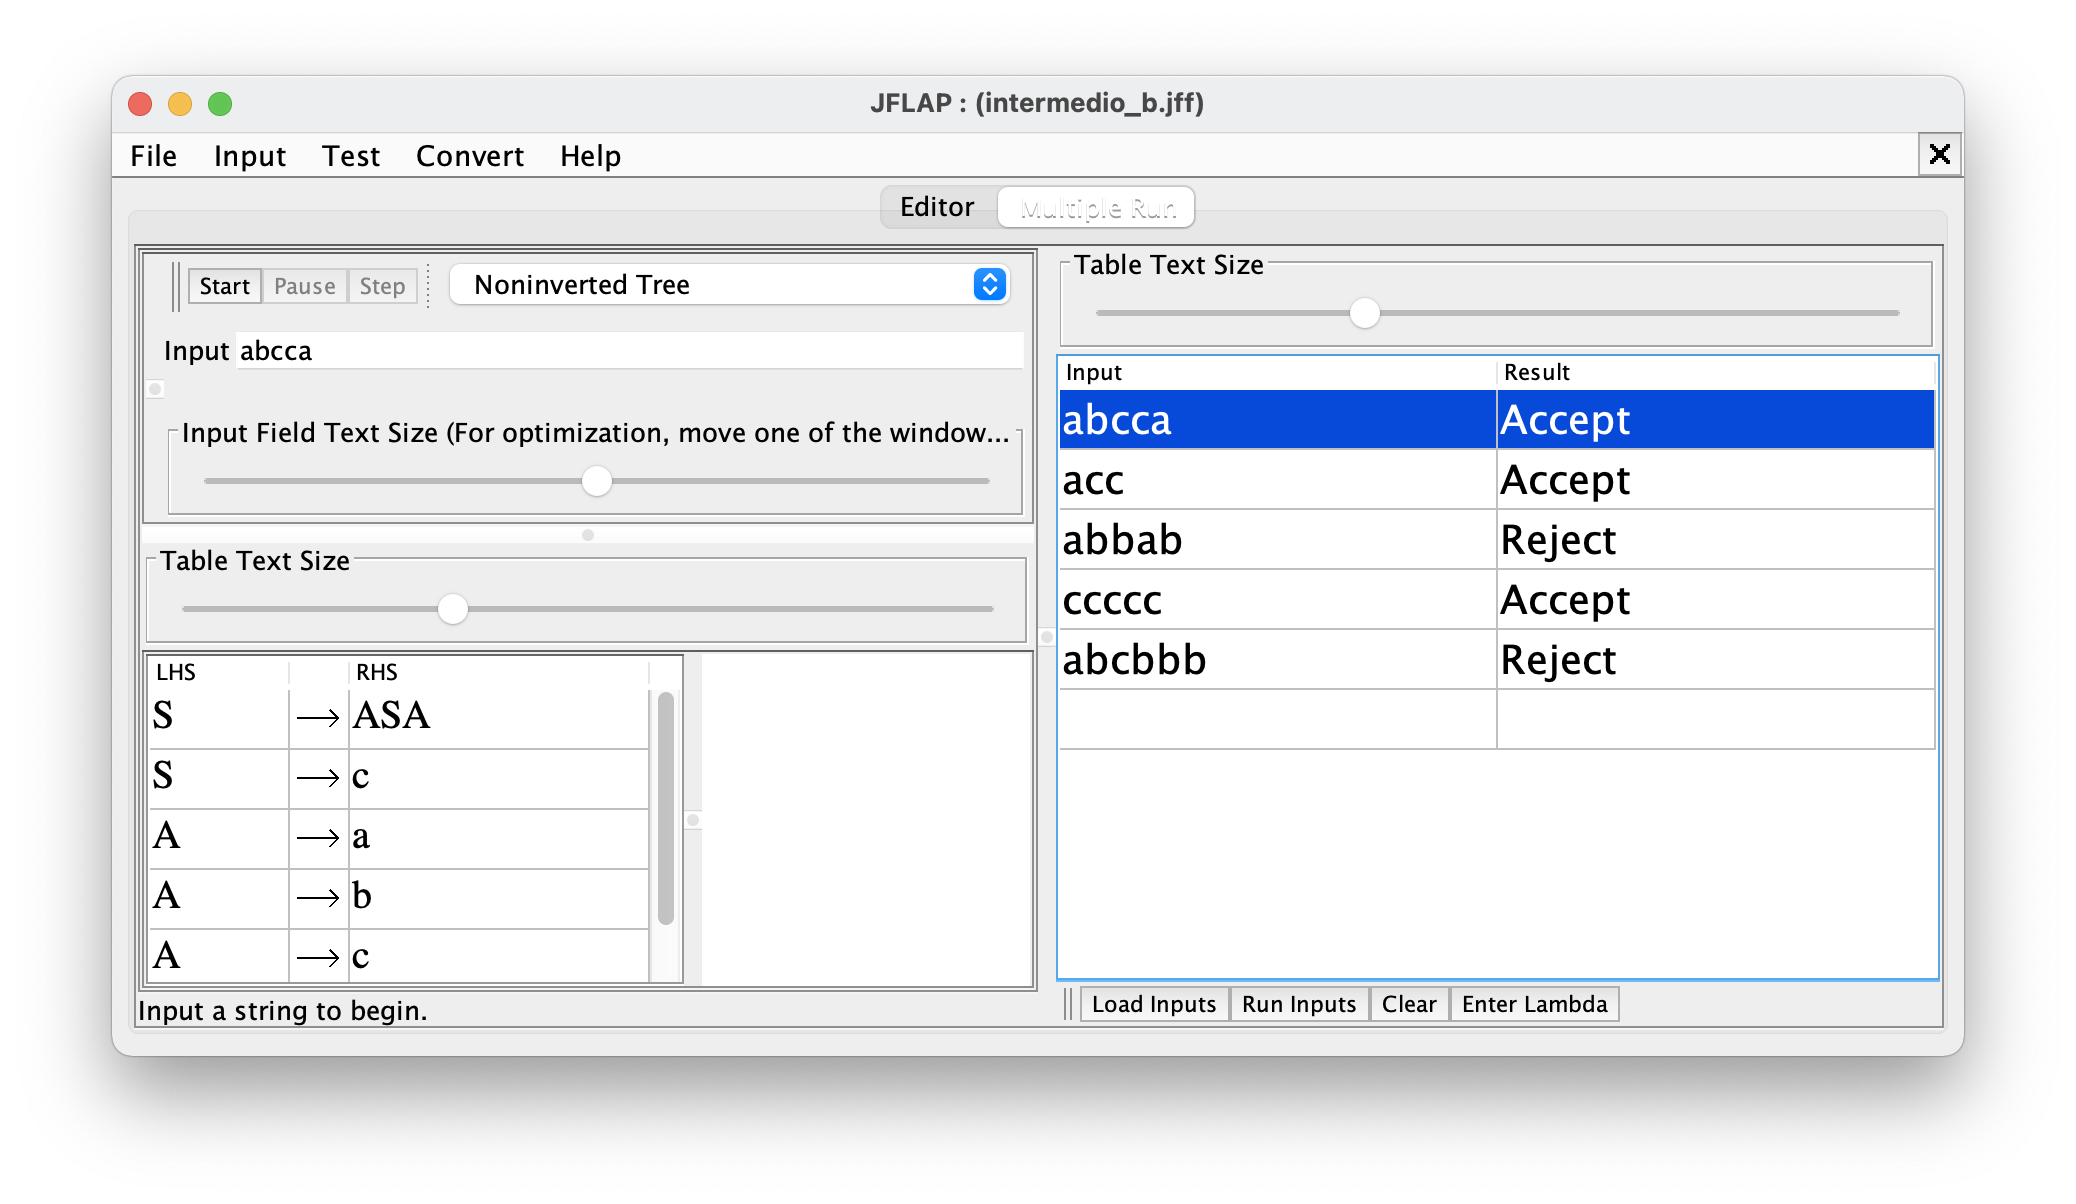
\includegraphics[scale=0.35]{../practica_1/images/intermedio_b.png} 
	\caption{Intermedio b en JFLAP} 
    \label{fig:intermedio_b}
\end{figure}

\textbf{c)}  $\{ u1^{n} \in \{0,1\}^{\ast} $ donde $\mid u \mid$ $= n \}$

\begin{figure}[H] 
	\centering
	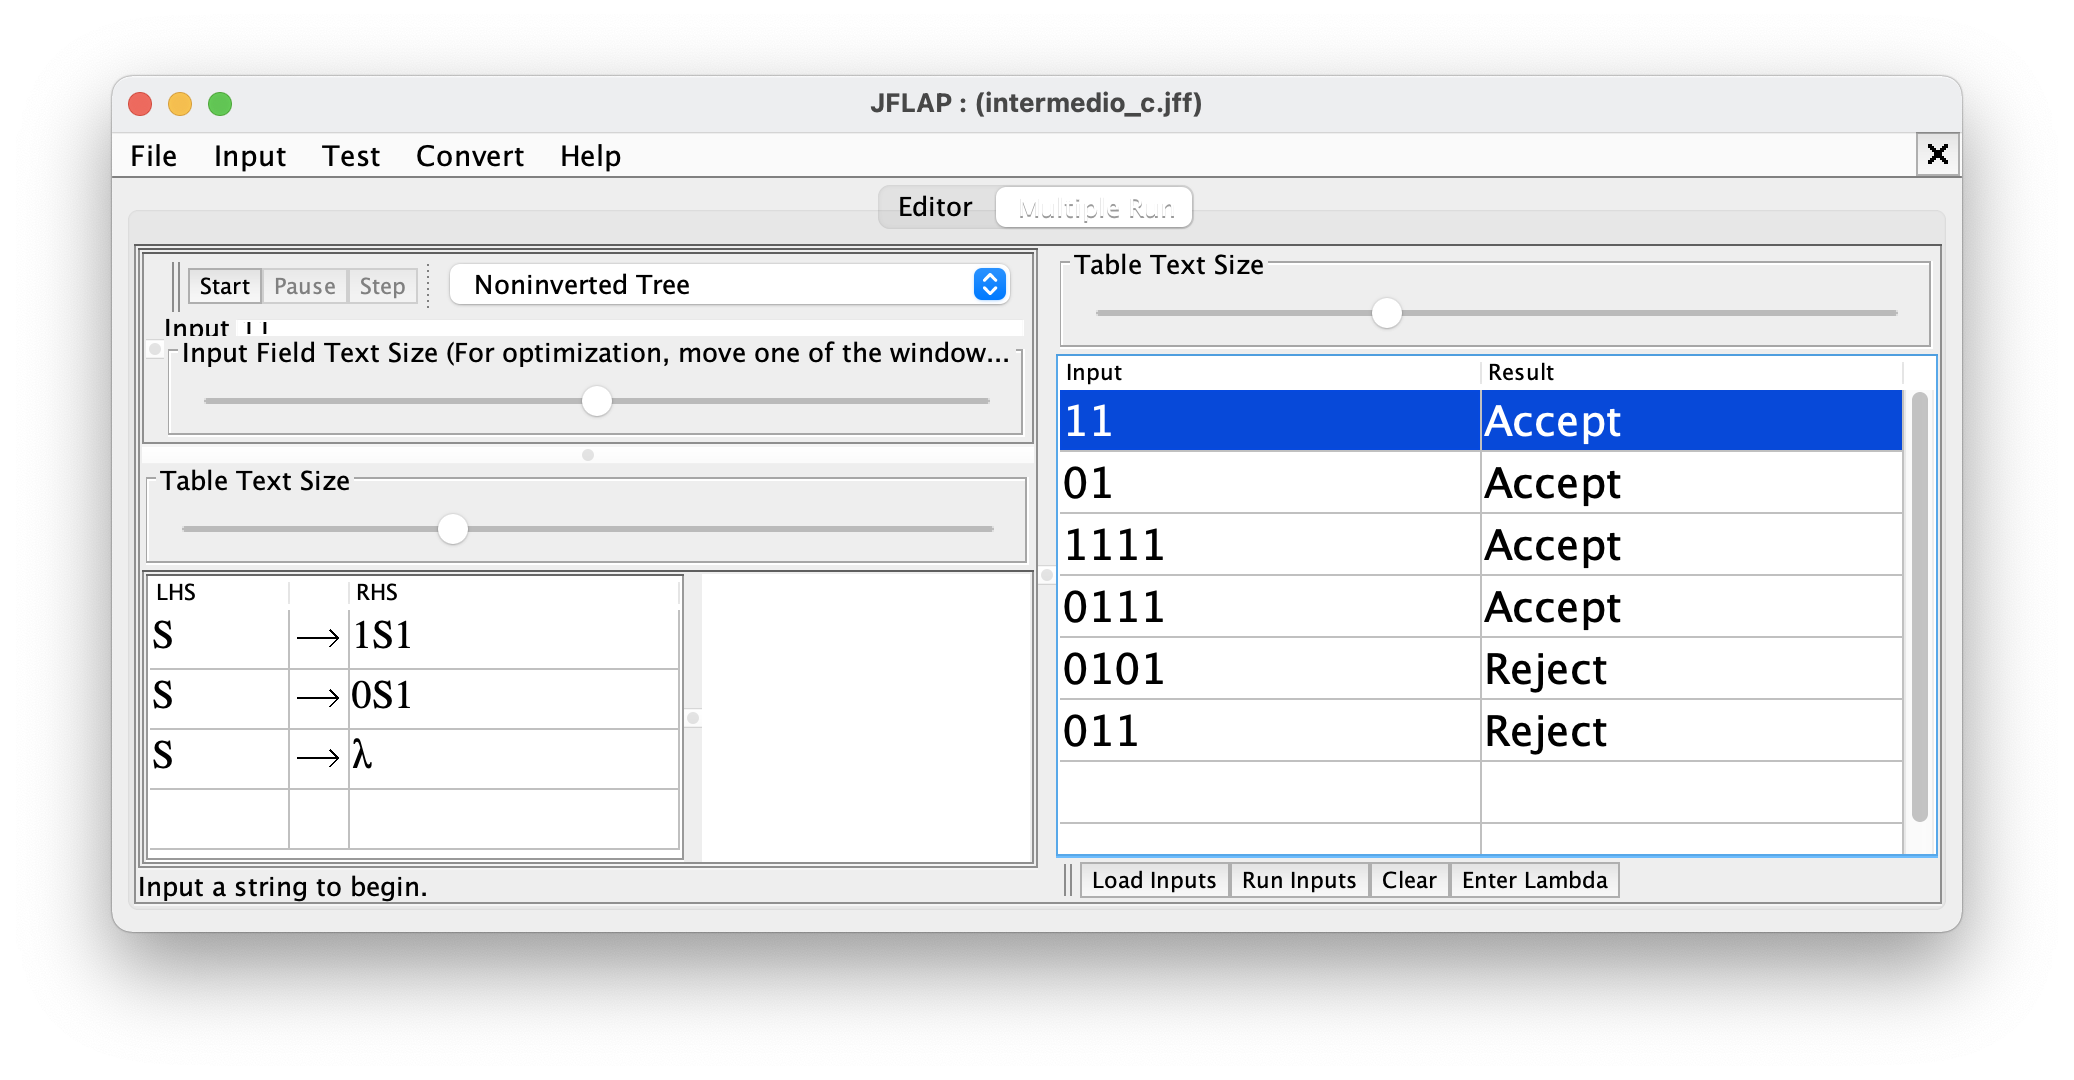
\includegraphics[scale=0.35]{../practica_1/images/intermedio_c.png} 
	\caption{Intermedio c en JFLAP} 
    \label{fig:intermedio_c}
\end{figure}

\textbf{d)}  $\{ a^{n} b^{n} a^{n+1} \in \{a,b\}^{\ast}$ con $n > 0\}$

\begin{figure}[H] 
	\centering
	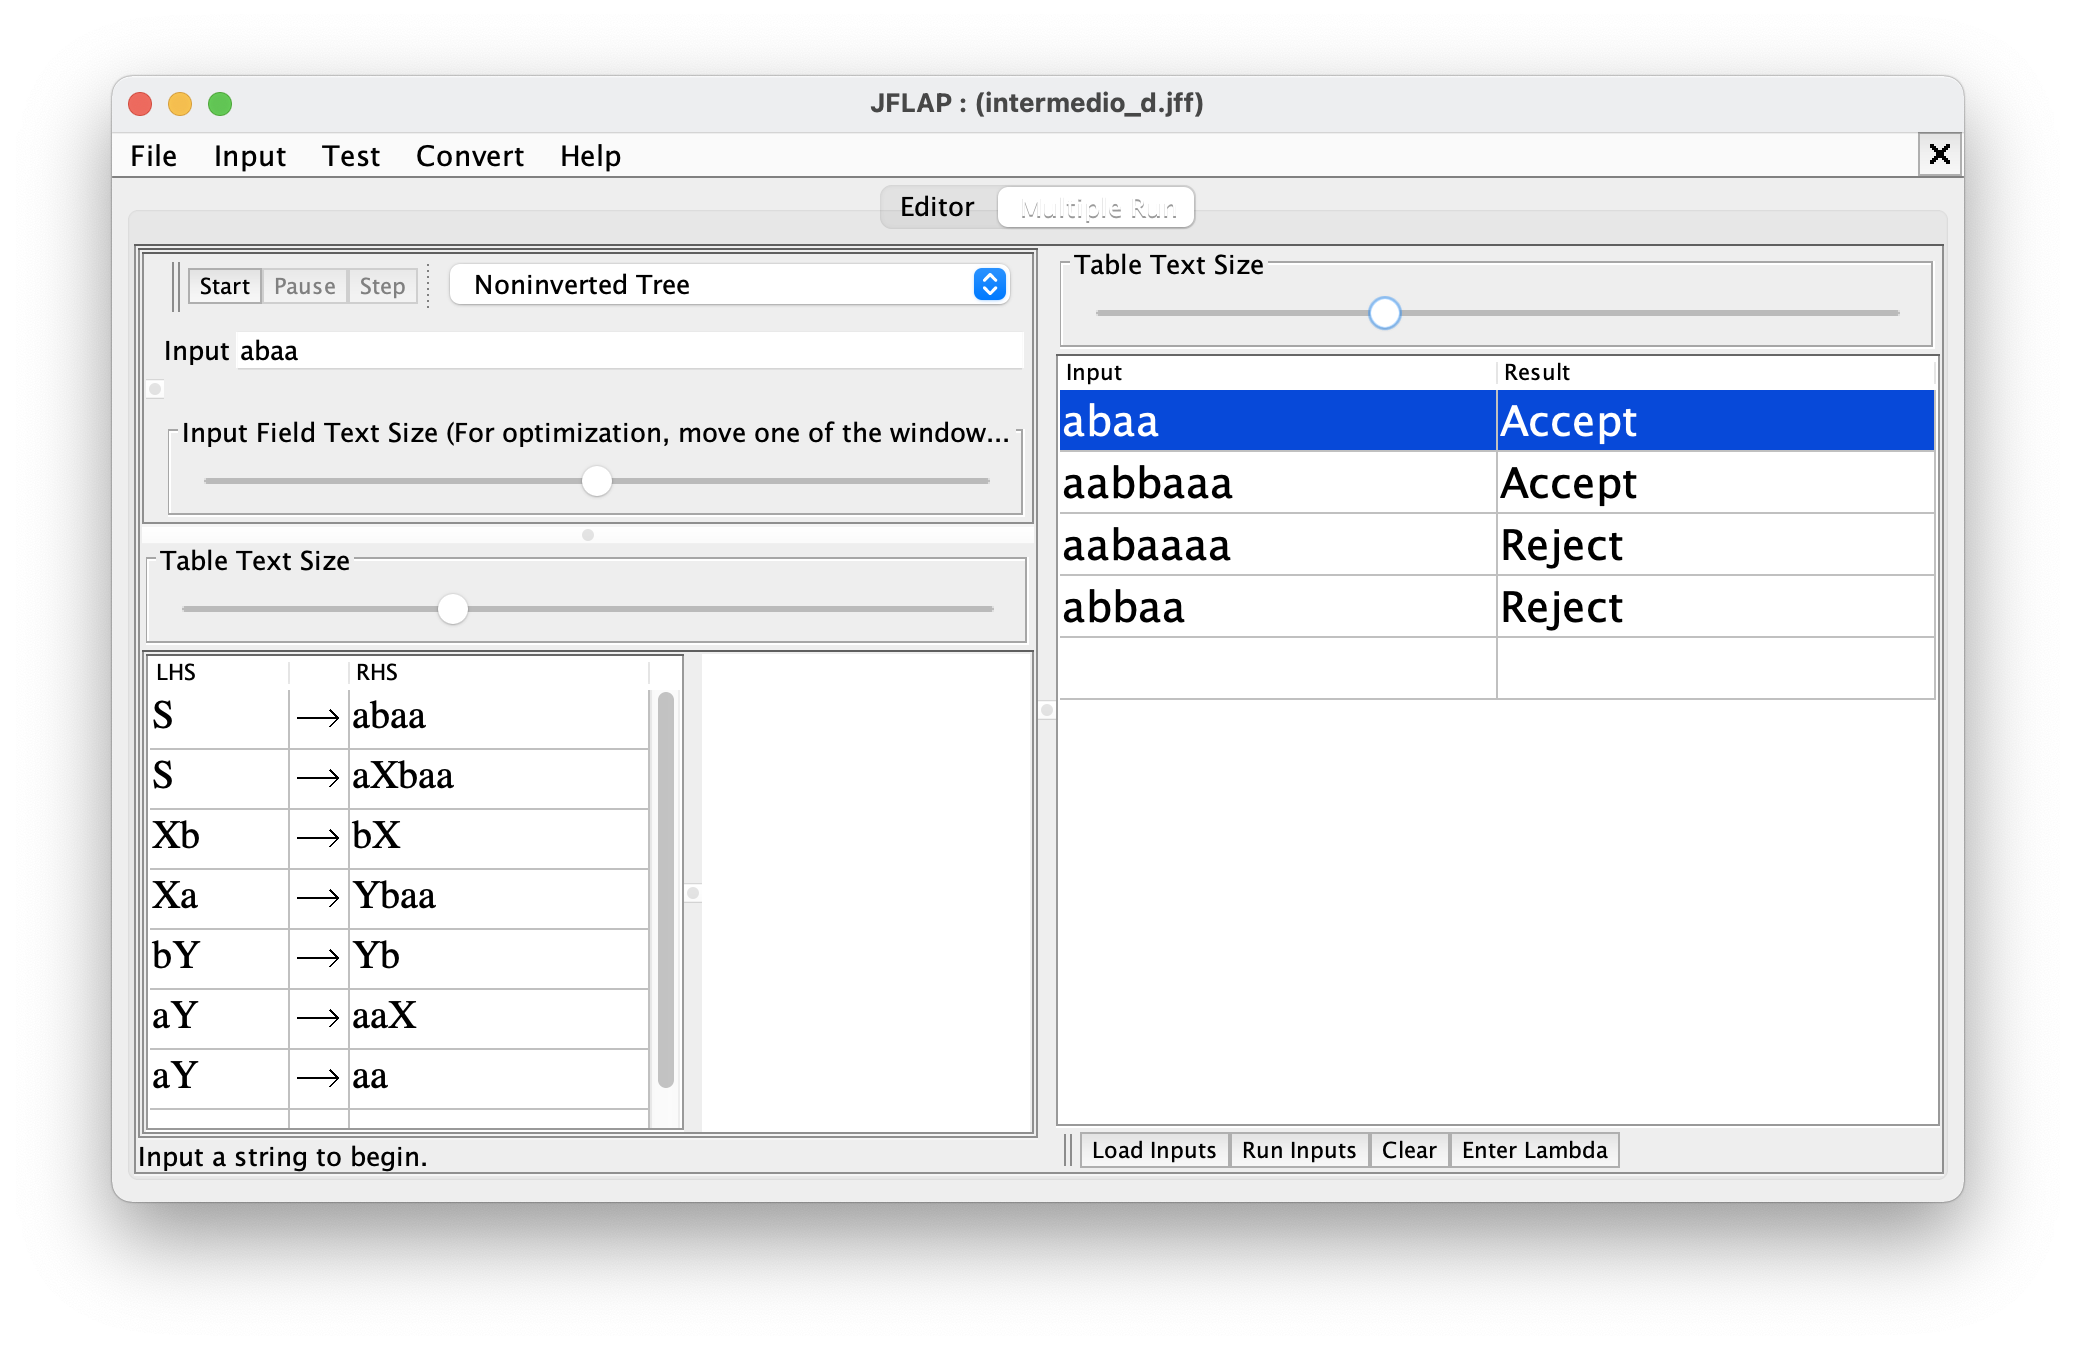
\includegraphics[scale=0.35]{../practica_1/images/intermedio_d.png} 
	\caption{Intermedio d en JFLAP} 
    \label{fig:intermedio_d}
\end{figure}

\subsection{Ejercicios Dificiles}

\textbf{a)}  $\{ u0v \in \{0,1\}^{\ast} $ tales que $u^{-1}$ es un prefijo de $v\}$

\begin{figure}[H] 
	\centering
	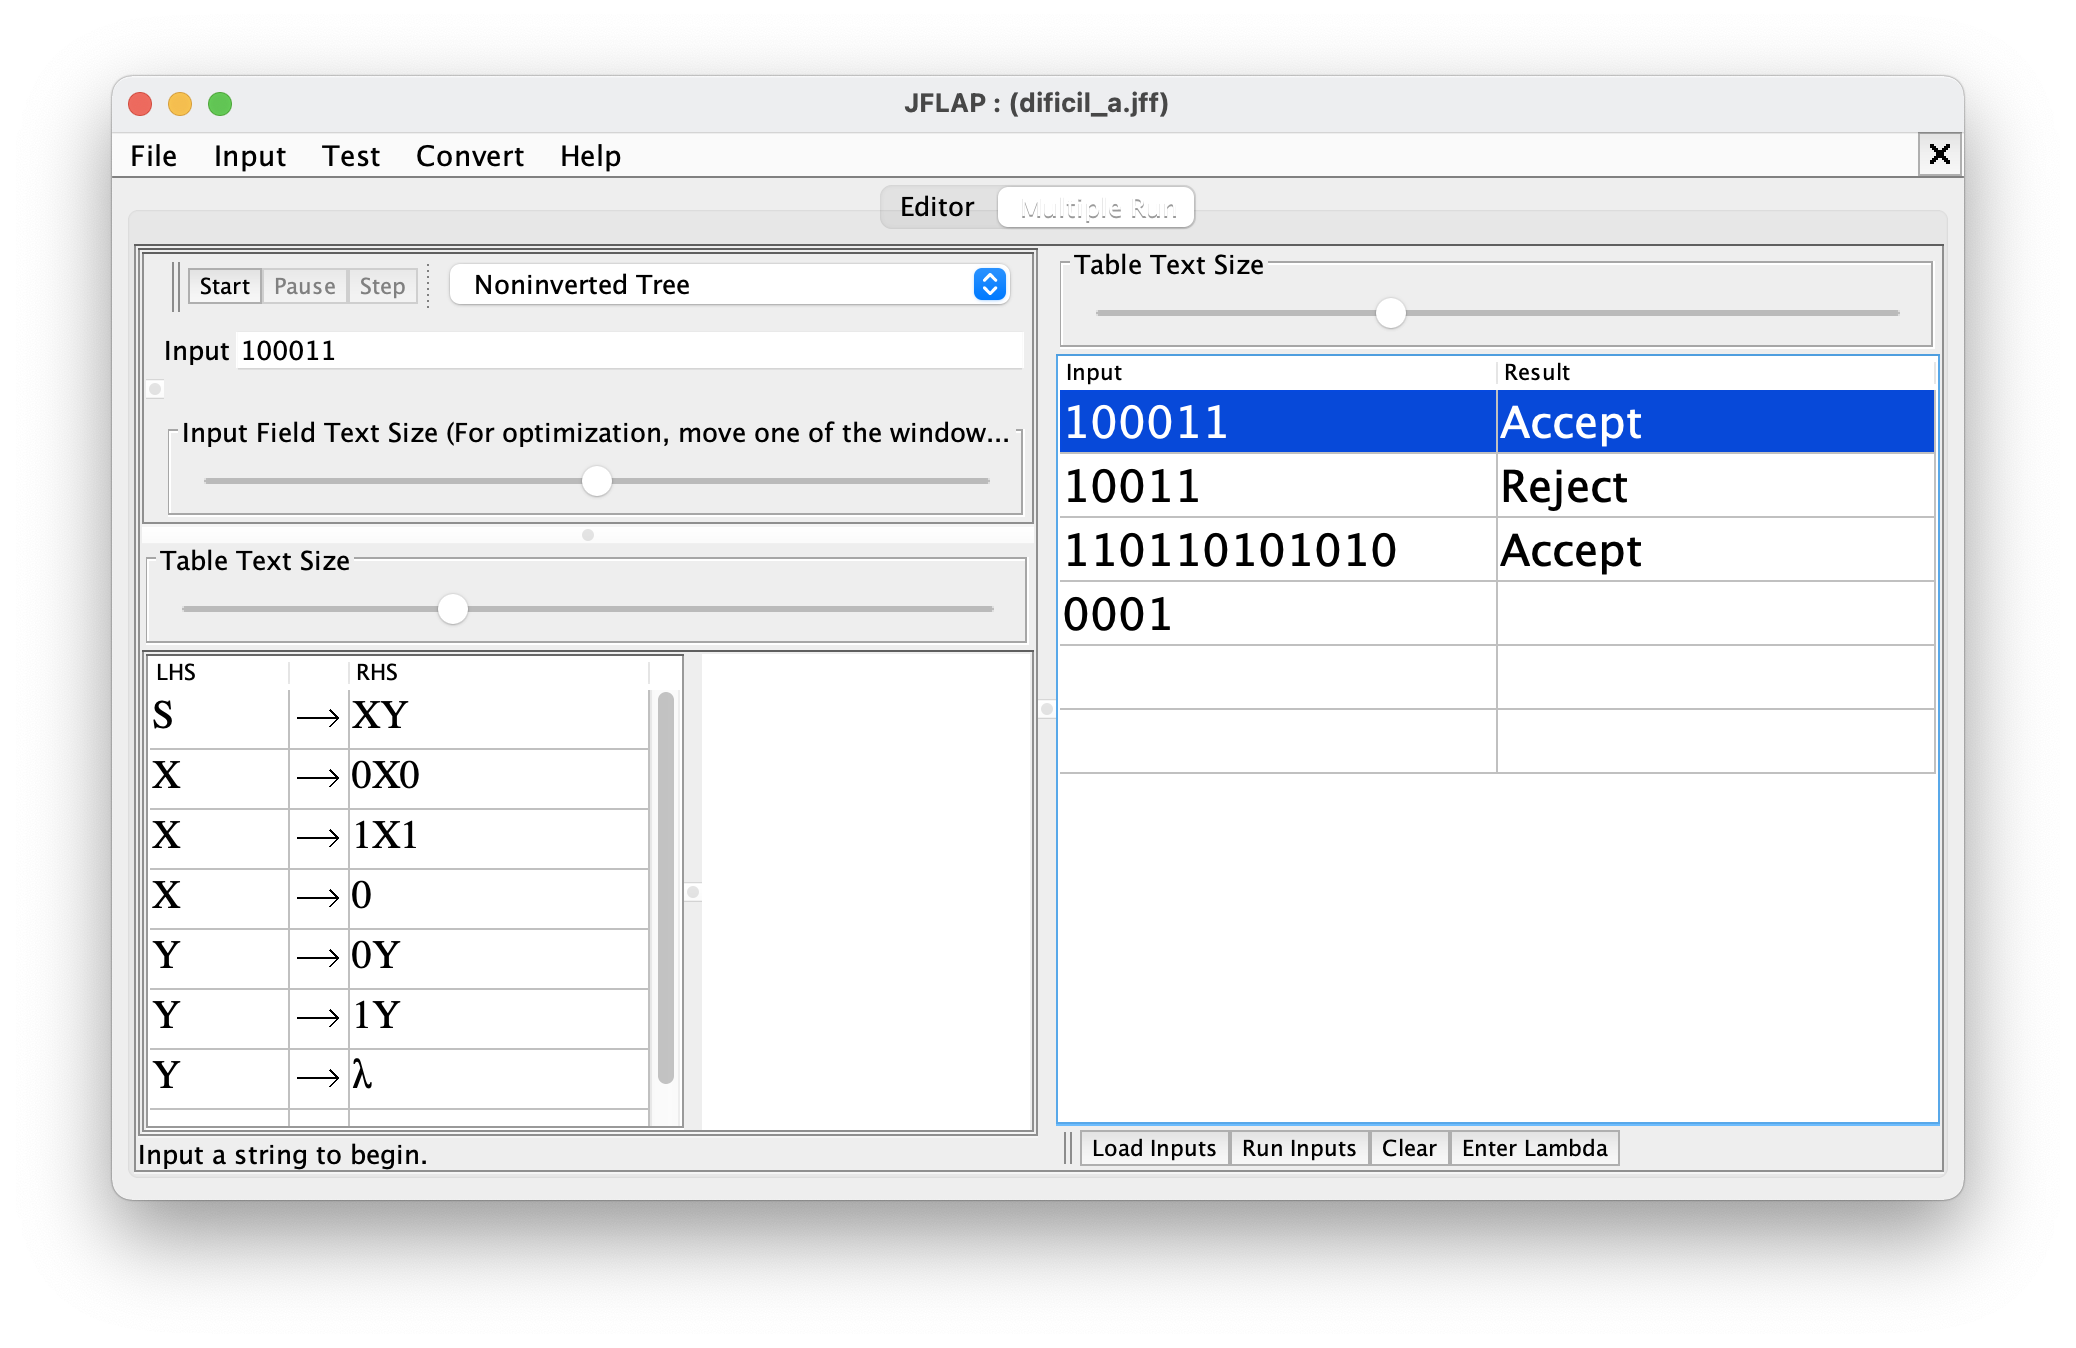
\includegraphics[scale=0.35]{../practica_1/images/dificil_a.png} 
	\caption{Dificil a en JFLAP} 
    \label{fig:dificil_a}
\end{figure}

\subsection{Ejercicios Extremos}

\textbf{a)}  $\{ ww$ con $w \in \{0,1\}^{\ast}\}$

\begin{figure}[H] 
	\centering
	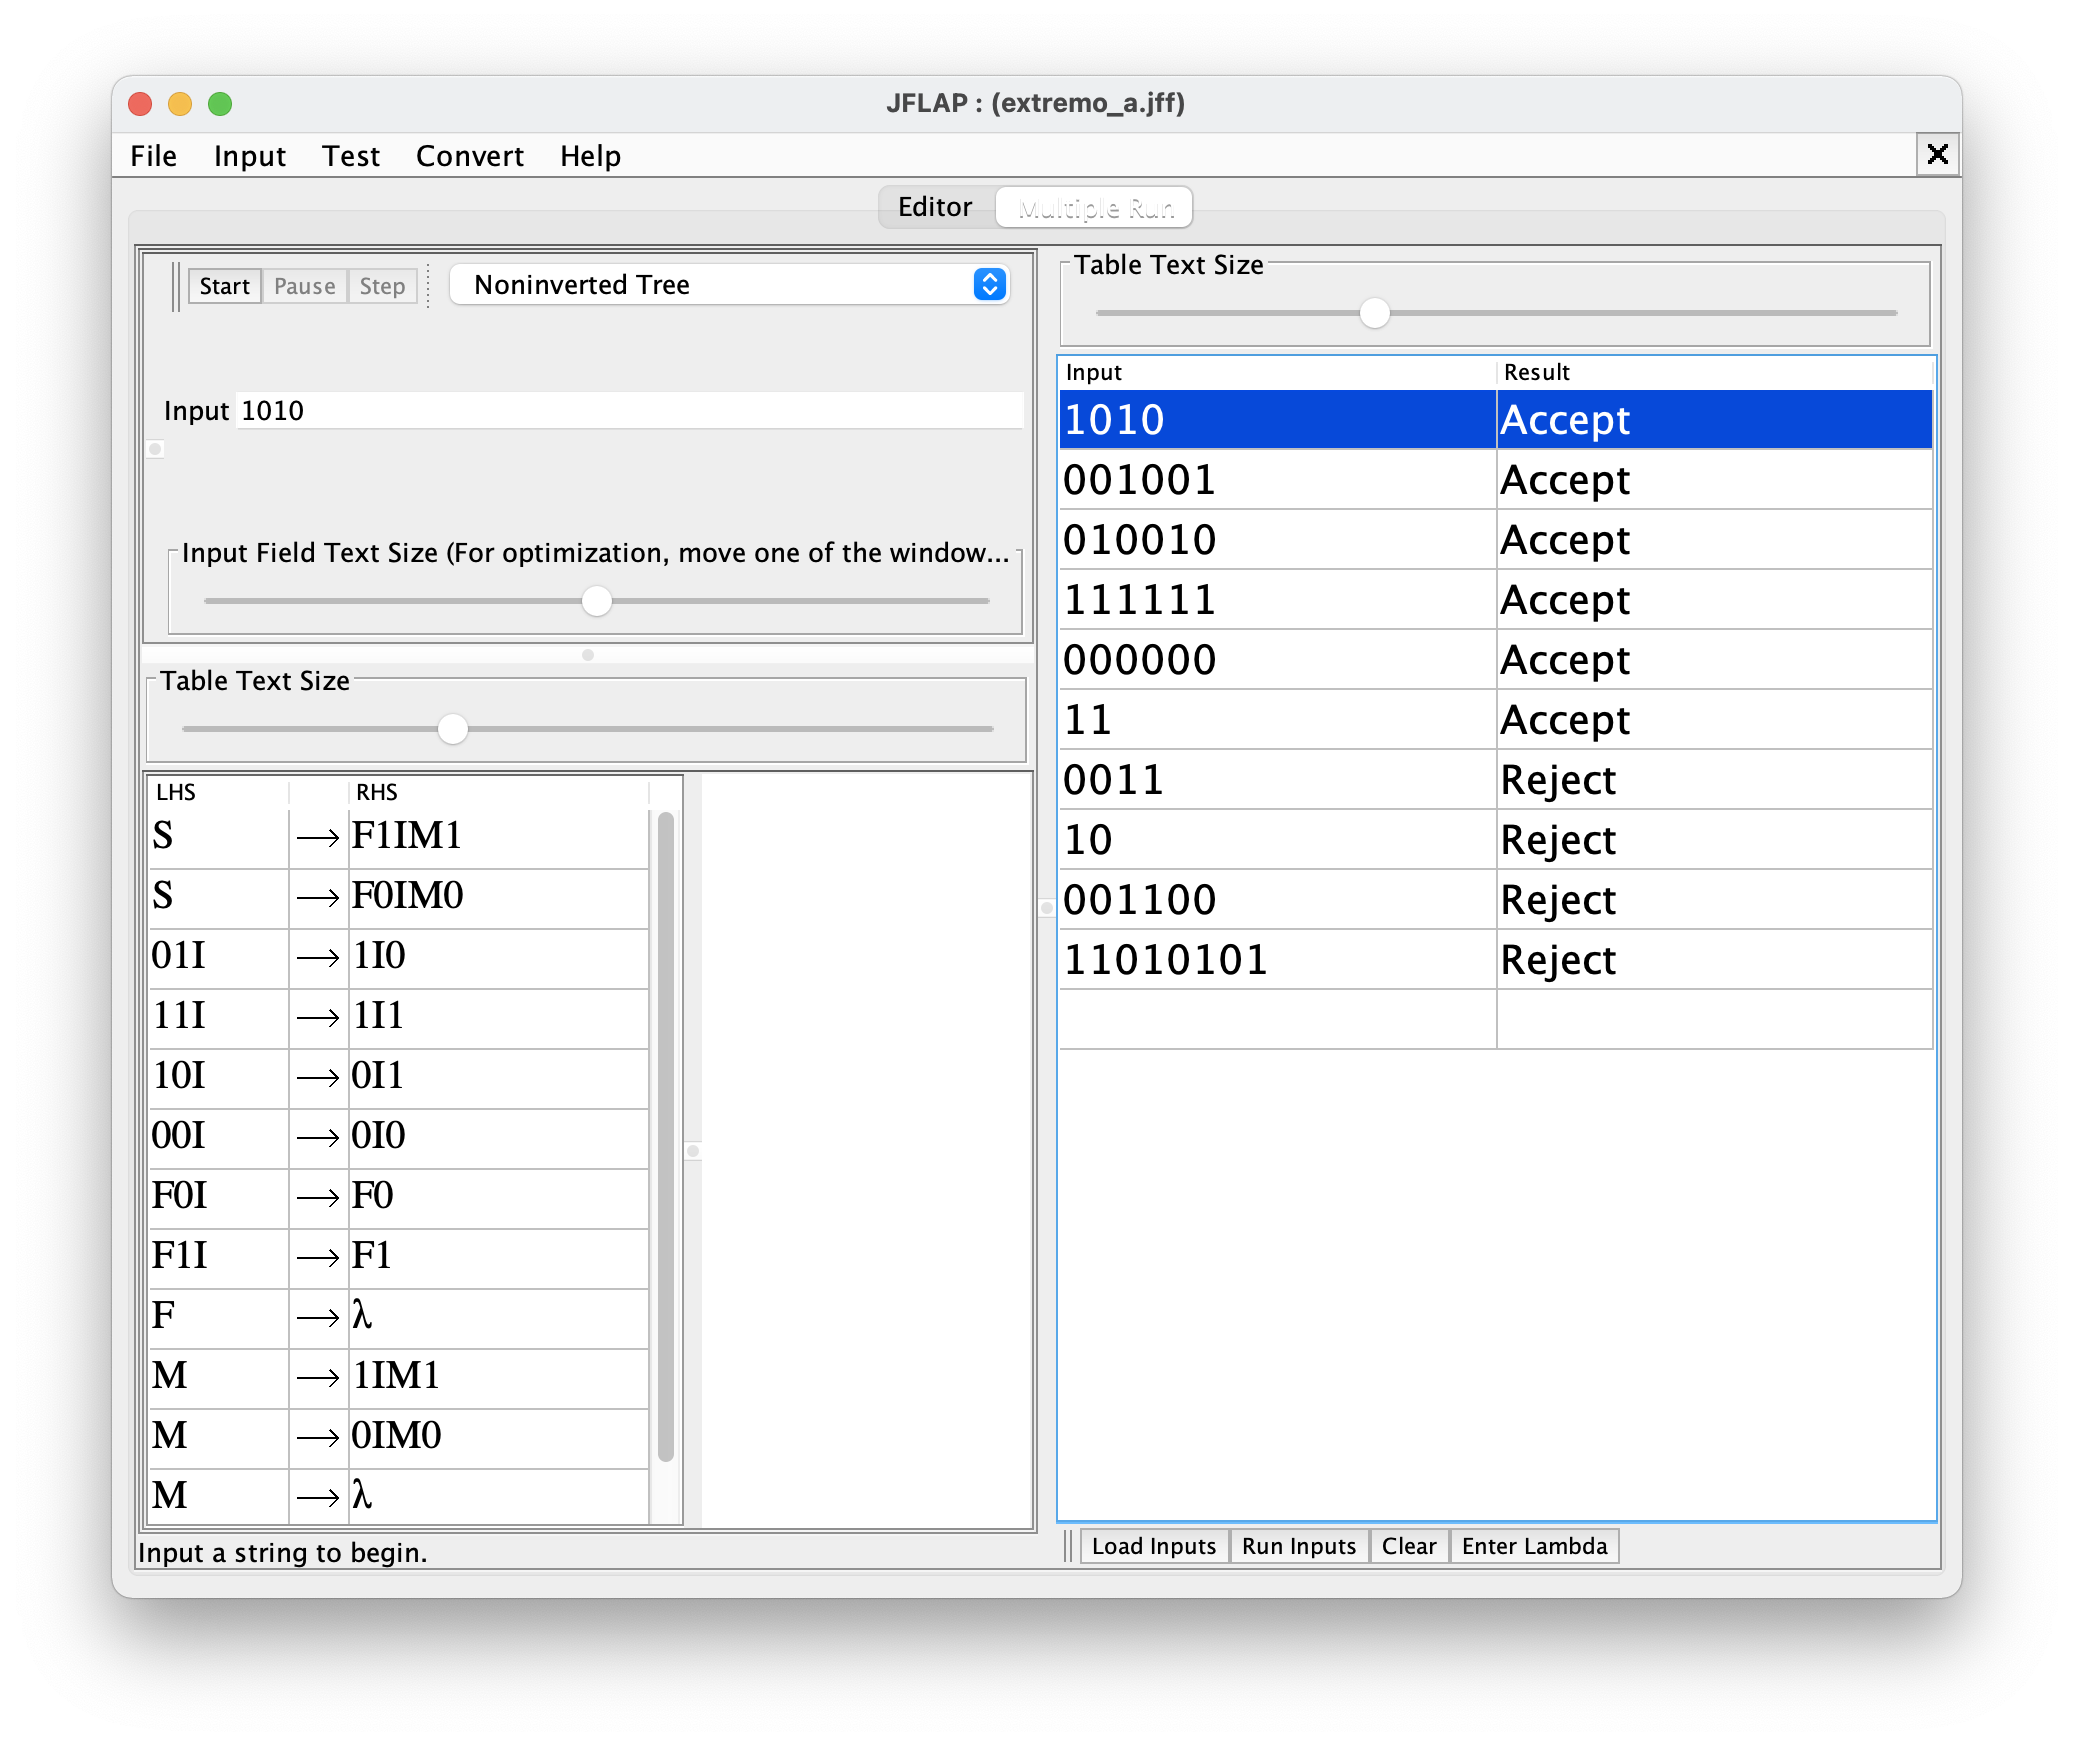
\includegraphics[scale=0.35]{../practica_1/images/extremo_a.png} 
	\caption{Extremo a en JFLAP} 
    \label{fig:extremo_a}
\end{figure}

\section{Practica 2 - Analizador Léxico}

\section{Practica 3 - Codificador-Decodificador}


\end{document}
